\RequirePackage{amsthm} %https://tex.stackexchange.com/questions/687324/unknown-theoremstyle-warning-with-springer-nature-template
\documentclass[sn-mathphys-num,iicol]{sn-jnl}

%\usepackage{sn-jnl.sty}
\usepackage{graphicx}%
\usepackage{multirow}%
\usepackage{amsmath,amssymb,amsfonts}%
\usepackage{amsthm}%
\usepackage{physics}
\usepackage{siunitx}
\usepackage{mathrsfs}%
\usepackage[title]{appendix}%
\usepackage{xcolor}%
\usepackage{textcomp}%
\usepackage{manyfoot}%
\usepackage{booktabs}%
\usepackage{algorithm}%
\usepackage{algorithmicx}%
\usepackage{algpseudocode}%
\usepackage{listings}%
\usepackage{newtxmath}%
\usepackage[tiny]{titlesec}%
%\usepackage[ngerman]{babel}
\usepackage{enumitem}
\usepackage{appendix}
\usepackage{subcaption}
\usepackage{afterpage}
\usepackage{hyperref} 

\theoremstyle{thmstyleone}
\newtheorem{theorem}{Theorem}
\newtheorem{proposition}[theorem]{Proposition}

\theoremstyle{thmstyletwo}
\newtheorem{remark}{Remark}

\theoremstyle{thmstylethree}
\newtheorem{definition}{Definition}

\raggedbottom

\newcommand{\td}{\text{d}}

\titleformat{\subsection}{}{\thesubsection}{1em}{\itshape}
\titleformat{\subsubsection}{}{\thesubsubsection}{1em}{\itshape}

\begin{document}
        
\title[]{Particle Detectors and Instrumentations}
\subtitle{Observation of Multiple Scattering}
\author*[1]{\fnm{Jonas} \sur{Wortmann}}\email{s02jwort@uni-bonn.de}
\author*[1]{\fnm{Marc} \sur{Hauer}}\email{s65mhaue@uni-bonn.de}
\author*[1]{\fnm{Pitt} \sur{Düster}}\email{s15pdues@uni-bonn.de}
\author*[1]{\fnm{Pouya} \sur{Dehghanfar}}\email{s28pdehg@uni-bonn.de}
\affil*[1]{Rheinische Friedrich--Wilhelms--Universität, Bonn}

\maketitle

\section{Introduction}
% In order to observe multiple scattering of electrons in aluminium and copper, a micromegas detector is used and tested with cosmic muon rays. Therefore a trigger logic is build with scintillators to select significant events.
% For a detailed observation of the multiple scattering, an electron beam provided by the ELSA accelerator will be used. This allows to compare the scattering behavior of electrons as they travel through aluminium and copper targets. To extend the analysis, targets of different thicknesses and a fixed distance between detector and target will be studied.  

When electrons pass through a material they undergo multiple scattering.
This process is observed with a micromegas detector for an electron beam hitting different materials with varying thicknesses.
To only count valid events a trigger logic is set up via two scintillators and logic modules, which is then tested with cosmic radiation.
The theoretical basis of the Highland formula for the angle deviation in multiple scattering is verified with a linear regression to show the correlation between the experimentally and theoretically calculated values.

%-----------------------------------------------------------------------------------------------------------------------------

\section{Theory}\label{sec:theory}
\subsection{Micromegas Detector}\label{subsec:theory_micromegas}
The Micromegas detector is a gaseous particle detector primarily used to detect ionizing radiation.
As shown in \autoref{fig:readout}, the detector consists of two main regions. 

The first region is the drift region, typically about \SI{5}{\milli\meter} thick.
A cathode is placed at the top and held at a negative voltage to establish a uniform electric field.
%pointing downward.
This field pulls negatively charged particles toward the micromesh. 
The drift region is filled with a noble gas mixture Ar/CO$_2$, which facilitates the ionization of the gas when a charged particle passes through. 
The ionization process liberates electrons. 
Because they do not attach to noble gases they can travel freely toward the mesh. 

The second region is the amplification region, which is significantly thinner, approximately \SI{128}{\micro\meter}. 
It is separated from the drift region by a woven micromesh, a metallic grid made of \SI{18}{\micro\meter} diameter stainless steel wires, with a density of \SI{157}{wires\per\cm}, resulting in an optical transparency of about 40\%.
An electric field of about \SI{500}{\volt\per\centi\meter} is applied between the cathode an the mesh, while a much stronger field of around \SI{70000}{\volt\per\centi\meter} is present between the mesh and the anode strips. 
This high field is due to the small gap and causes incoming electrons to gain enough energy to further ionize the gas, leading to an avalanche multiplication of electrons. 
The ions, on the other hand, drift upward the mesh. 
The electrons are collected by the anode strips, which make up the readout plate and results in a measurable electrical signal. 
Those regions together with the readout plane form the active area of the detector which is about \SI{100}{\centi\meter^2}.
\begin{figure}
  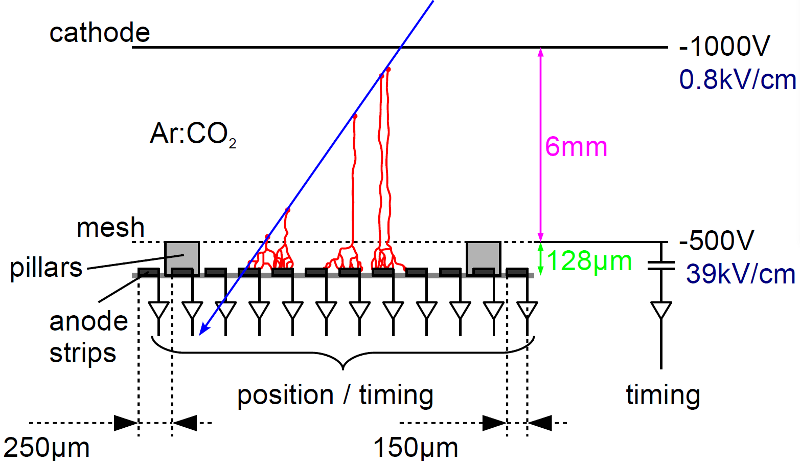
\includegraphics[width=\linewidth]{figures/detector_readout.png}
  \caption{Setup of micromegas detector with a two dimensional readout \cite{Micromegas}}
  \label{fig:readout}
\end{figure}

\subsection{Multiple Scattering}\label{subsec:theory_scattering}
When a charged particle travels through a material, it undergoes numerous interactions with the Coulomb potential of the nucleus resulting in small angle deflections.
The overall effect of those deflections is known as multiple scattering. 

The distribution of the resulting deflection angles is approximately Gaussian in the central region. 
This statistical treatment of deflections allows one to describe the angular distribution with a root mean square (RMS) scattering angle.
A formula to estimate the RMS projected scattering angle is given by the Highland approximation \cite{Highland}
\begin{equation}\label{eq:Highland}
    \theta_0 = \frac{13.6\,\text{MeV}}{\beta cp} \, z \, \sqrt{\frac{x}{X_0}} \left[1 + 0.038 \ln\left(\frac{x}{X_0}\right)\right],
\end{equation}
where $\theta_0$ is the RMS scattering angle in the projected plane, $p$ is the momentum of the incident particle, $\beta$ is its velocity divided by the speed of light, $z$ is the charge number of the particle, $x$ is the thickness of the target material, and $X_0$ is the radiation length of the material.

The angular distribution of scattered particles, in the small-angle approximation, follows a Gaussian probability distribution centered around the initial direction of the particle beam \cite{Highland2}
\begin{equation}\label{eq:Gauss}
P(\theta) = \frac{1}{\sqrt{2\pi} \, \theta_0} \exp\left( -\frac{\theta^2}{2\theta_0^2} \right).
\end{equation}
In experimental setups, the angular spread caused by multiple scattering can be observed by placing a detector at a known distance $d$ from the target. 
Based on geometrical considerations it follows that \cite{Highland2}
\begin{equation}\label{eq:theta_exp}
\sigma = d \cdot \tan\left(\theta_{\text{exp}}\right)\qquad
\theta_{\text{exp}} = \arctan\left( \frac{\sigma}{d} \right).
\end{equation}
Increasing the distance $d$ between the target and the detector results in a proportional increase in the lateral spread making the distribution wider.
Changing the thickness $x$ of the target material has a direct impact. 
Since the RMS angle $\theta_0$ grows with $\sqrt{x}$, a thicker target leads to broader angular distributions due to more scattering events. 
Likewise, decreasing the radiation length $X_0$ increases $\theta_0$, again broadening the Gaussian spread. 
Therefore, materials with shorter radiation lengths cause more significant angular deflection over the same thickness.

%-----------------------------------------------------------------------------------------------------------------------------

\section{Cosmic Data}
\subsection{Measuring of Detector Specifications} \label{subsec:detector_specific} % structure? 
For a deeper understanding of the structure of a micromegas detector \cite{Micromega} the spare detector depicted in \autoref{fig:micromegas_closed} is disassembled.

%\begin{figure}
%  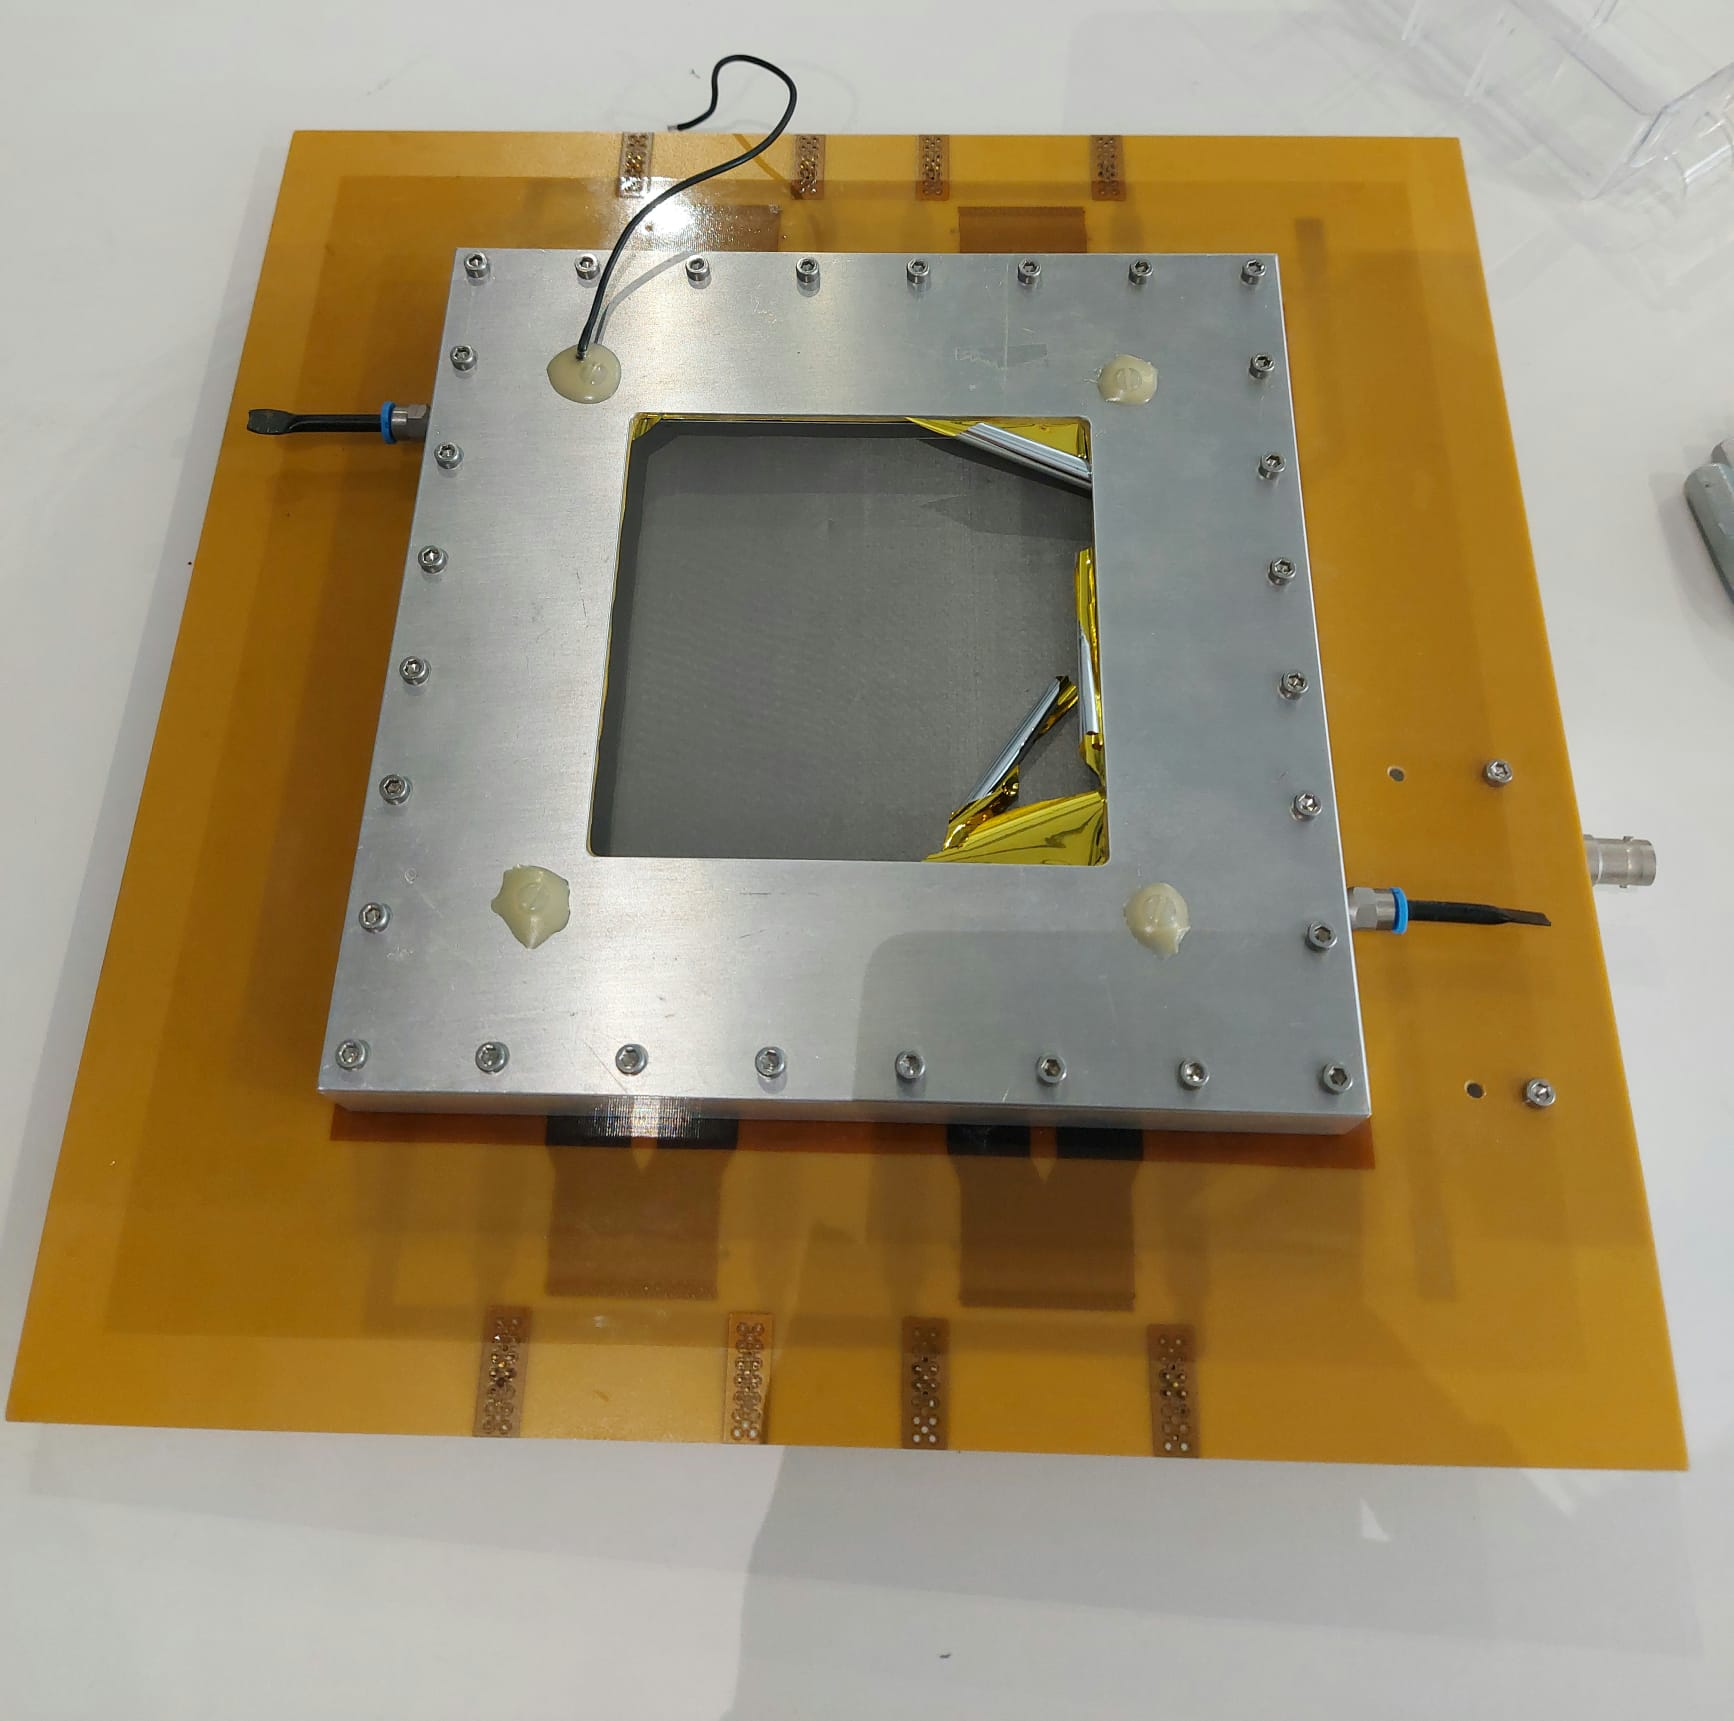
\includegraphics[width=\linewidth]{figures/micromegas_closed.jpeg}
%  \caption{Front of the spare micromegas detector}
%  \label{fig:micromegas_closed}
%\end{figure}

To access the inner part of the micromegas detector the screws on the top, and the upper part are removed.
Attached to the upper metal part is a mesh which is held by four plastic pillars as can be seen in \autoref{fig:micromegas_cover}.
This mesh is used as the cathode of the detector. 
The distance between the entry window and the cathode is measured to be \SI{1.0\pm.1}{\centi\meter} and the diameter of the cathode to be \SI{11\pm.1}{\centi\meter}.
These measurements were done with a ruler and we therefore assumed an uncertainly of \SI{.1}{\centi\meter} on all measurements.

%\begin{figure}
%  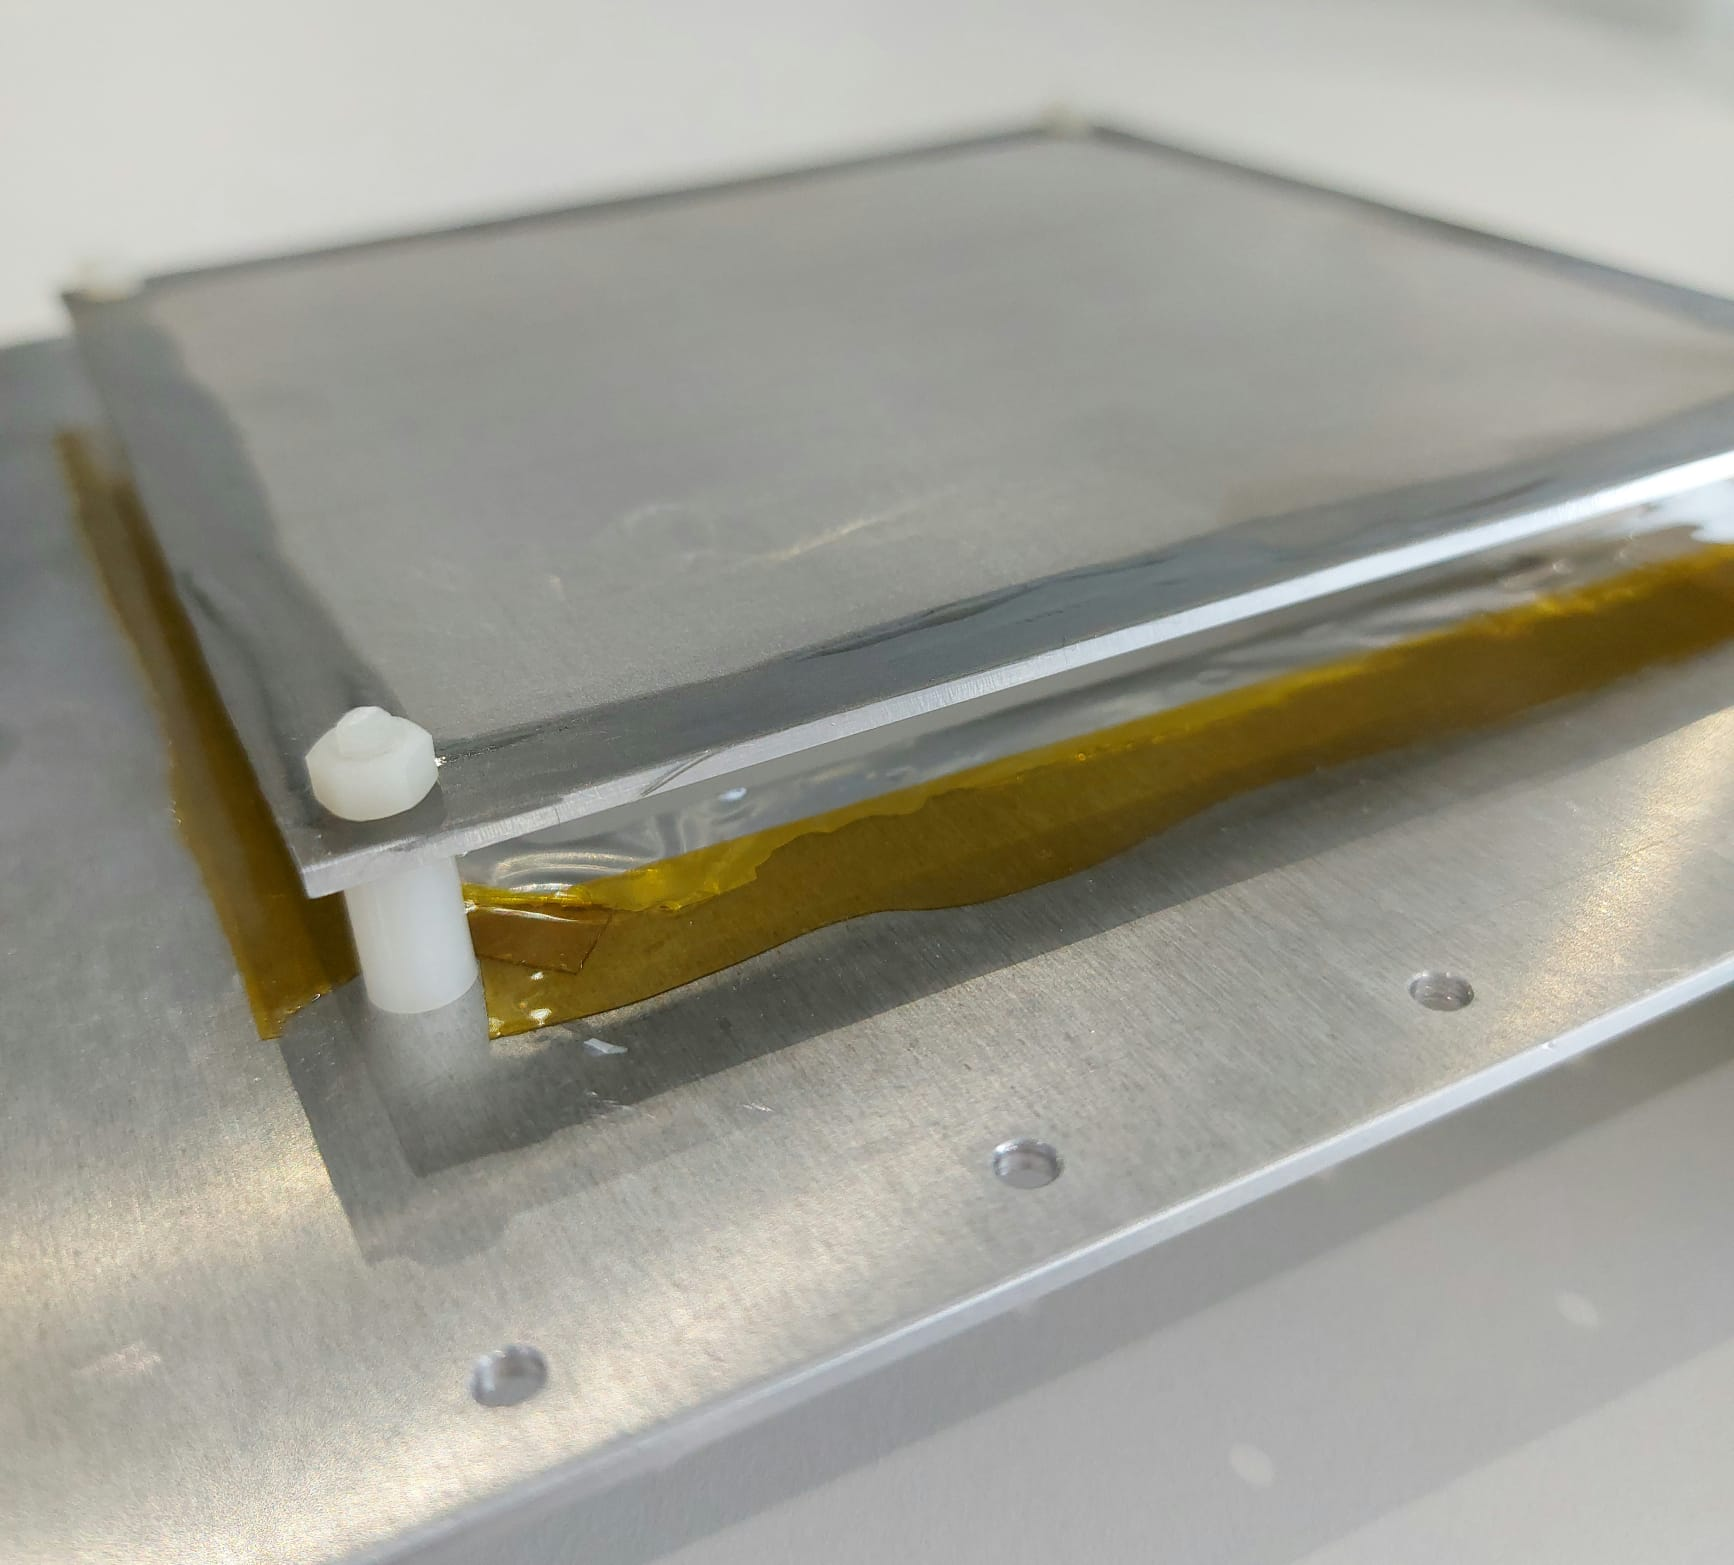
\includegraphics[width=\linewidth]{figures/micromegas_cover.jpeg}
%  \caption{Cathode mesh on the upper part of the micromegas}
%  \label{fig:micromegas_cover}
%\end{figure}

In \autoref{fig:micromegas_base} the inside of the detector is shown. 
The cathode was placed in the center gap.
At the bottom one can see the mesh of the detector, which is responsible for gas amplification as explained in \autoref{subsec:theory_micromegas}.
The inner diameter of the mesh is \SI{13.8\pm.1}{\centi\meter}.

%\begin{figure}
%  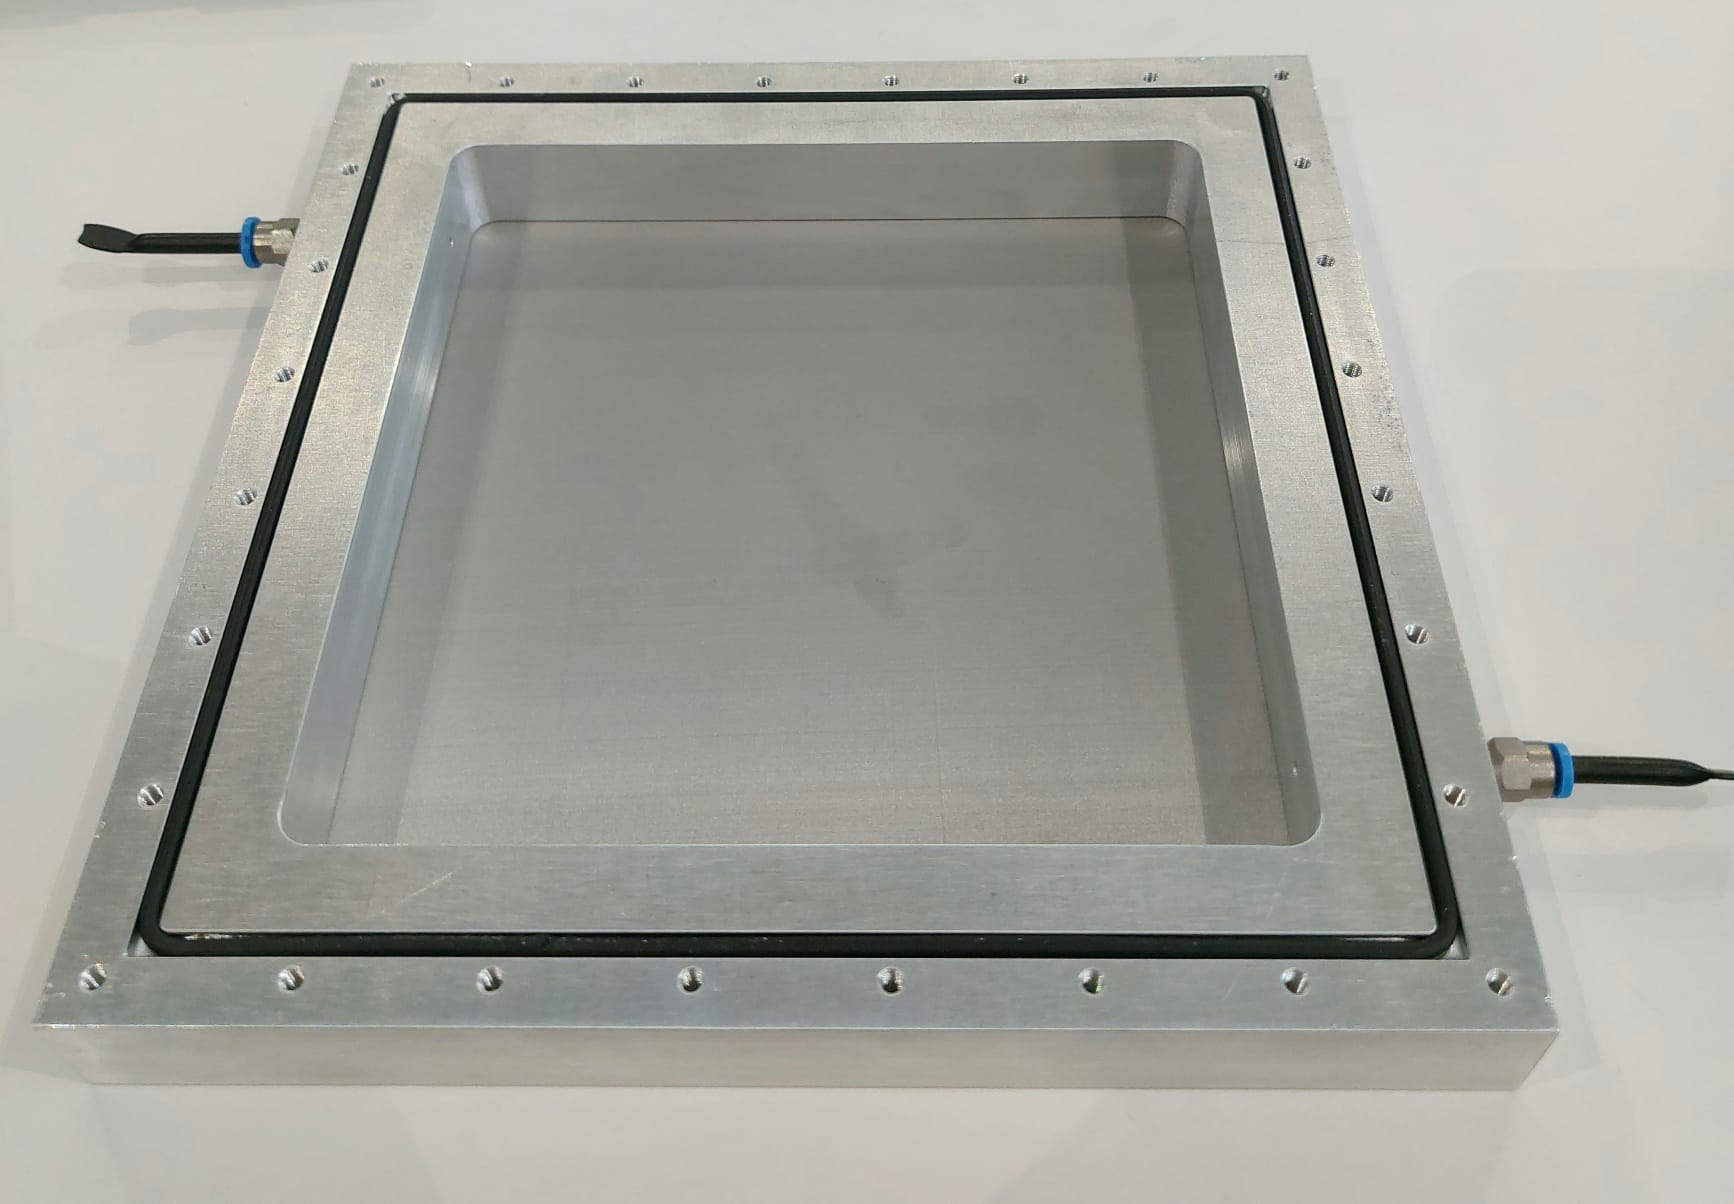
\includegraphics[width=\linewidth]{figures/micromegas_base_top.jpeg}
%  \caption{Bottom part of the micromegas with the mesh}
%  \label{fig:micromegas_base}
%\end{figure}

Below the mesh one can see the anode strips on the PCB wafer shown in \autoref{fig:micromegas_strips}.
The active area is measured to be \SI{10\pm1.4}{\cm^2} where the uncertainty is calculated by the Gaussian propagation of uncertainty.
One observes a grid-like structure of the anodes with width and height of one rectangle of $\SI{4\pm1}{\mm}\times\SI{5\pm1}{\mm}$.
One rectangle in this structure is connected with 10 wires.
This indicates that there are 10 strips per rectangle.
Therefore the true dimensions of one strip is $\SI{400\pm100}{\micro\meter}\times\SI{500\pm100}{\micro\meter}$.

%\begin{figure}
%  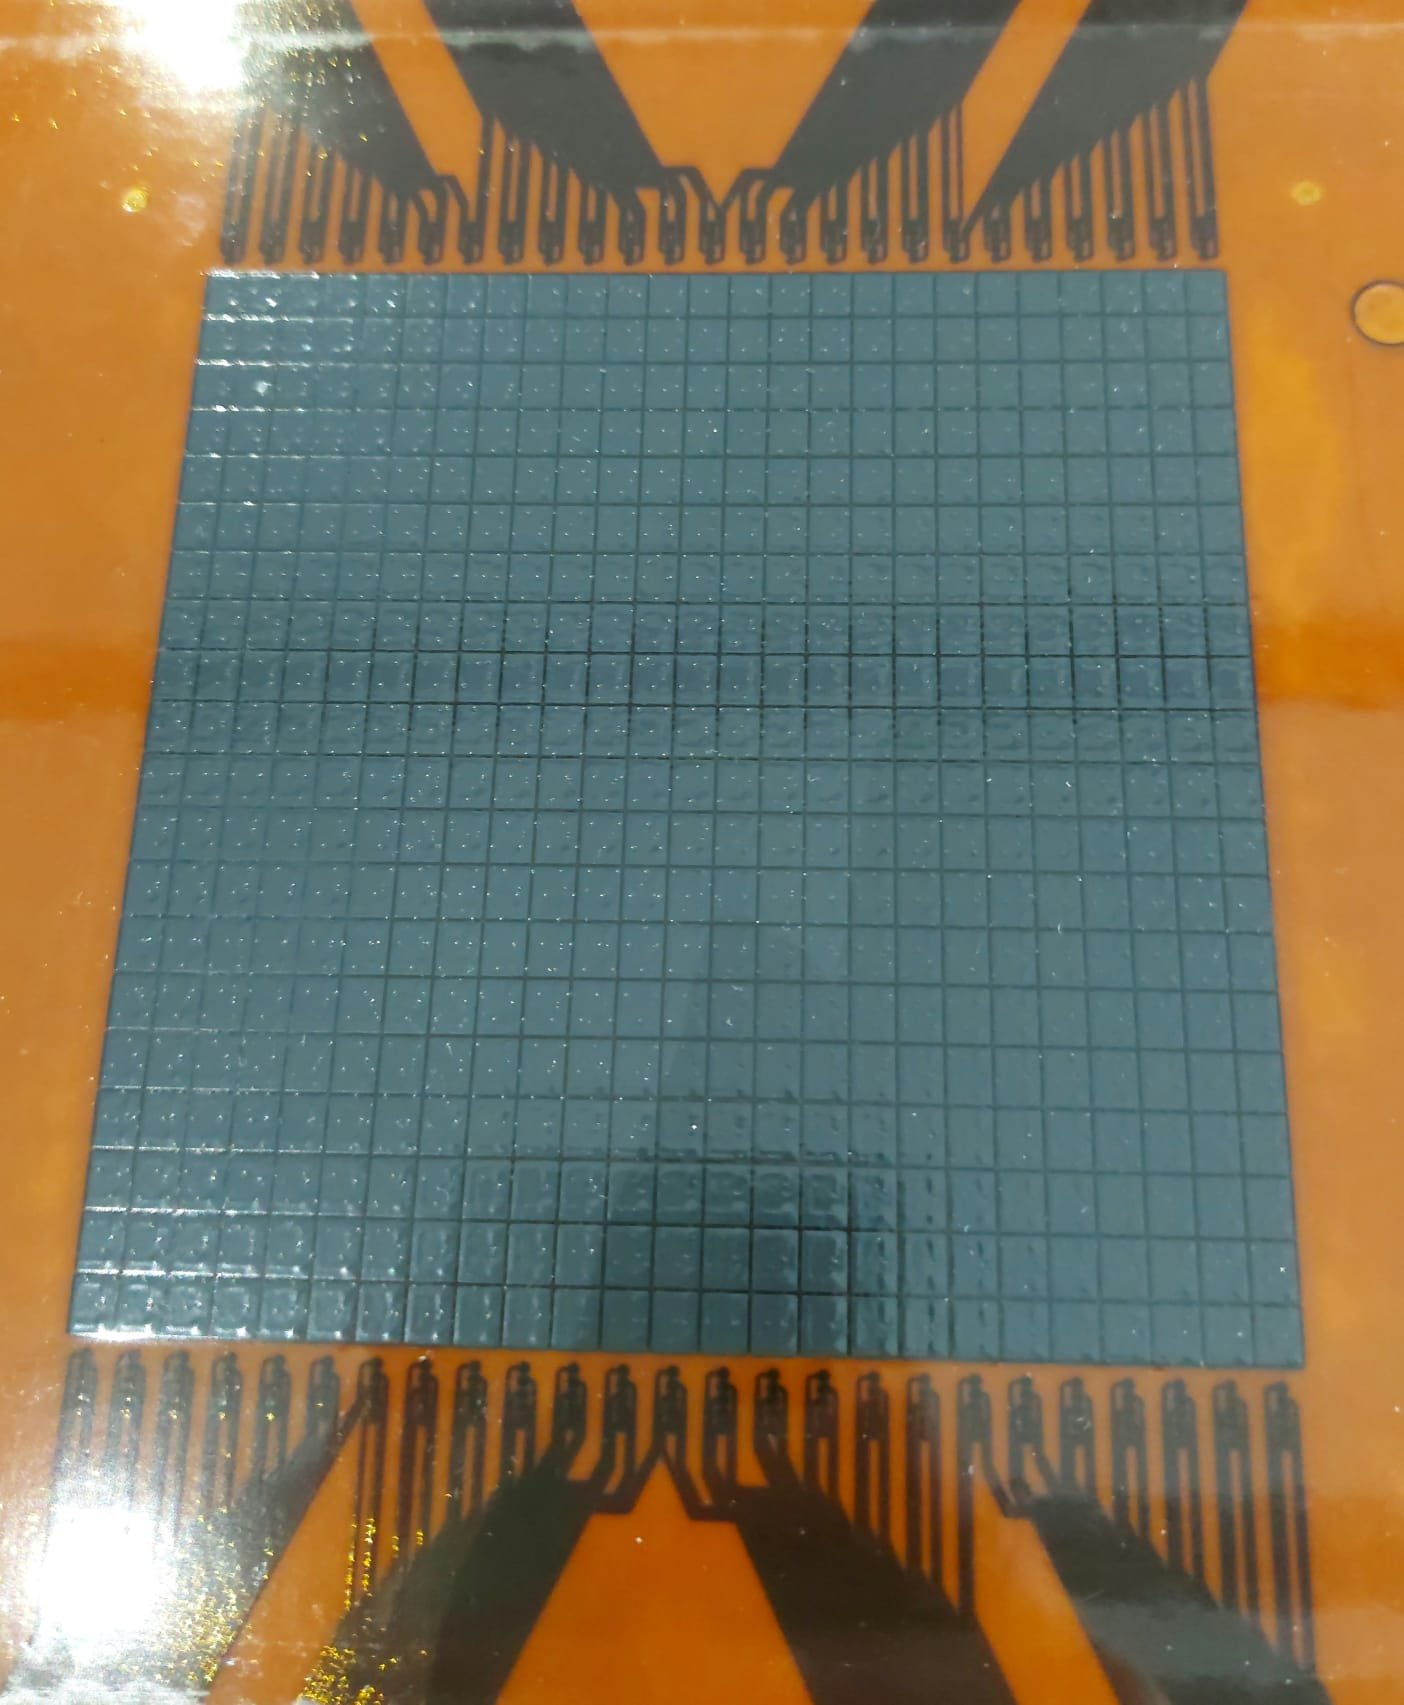
\includegraphics[width=\linewidth]{figures/micromegas_strips.jpeg}
%  \caption{Grid-like structure of the anode strips}
%  \label{fig:micromegas_strips}
%\end{figure}

\subsection{Experimental Setup}
To observe cosmic muon rays, a micromegas detector is set up horizontally between two scintillators \cite{Scint}.
These scintillators are overlapping and positioned as shown in \autoref{fig:setup_ROT}.

\begin{figure}
  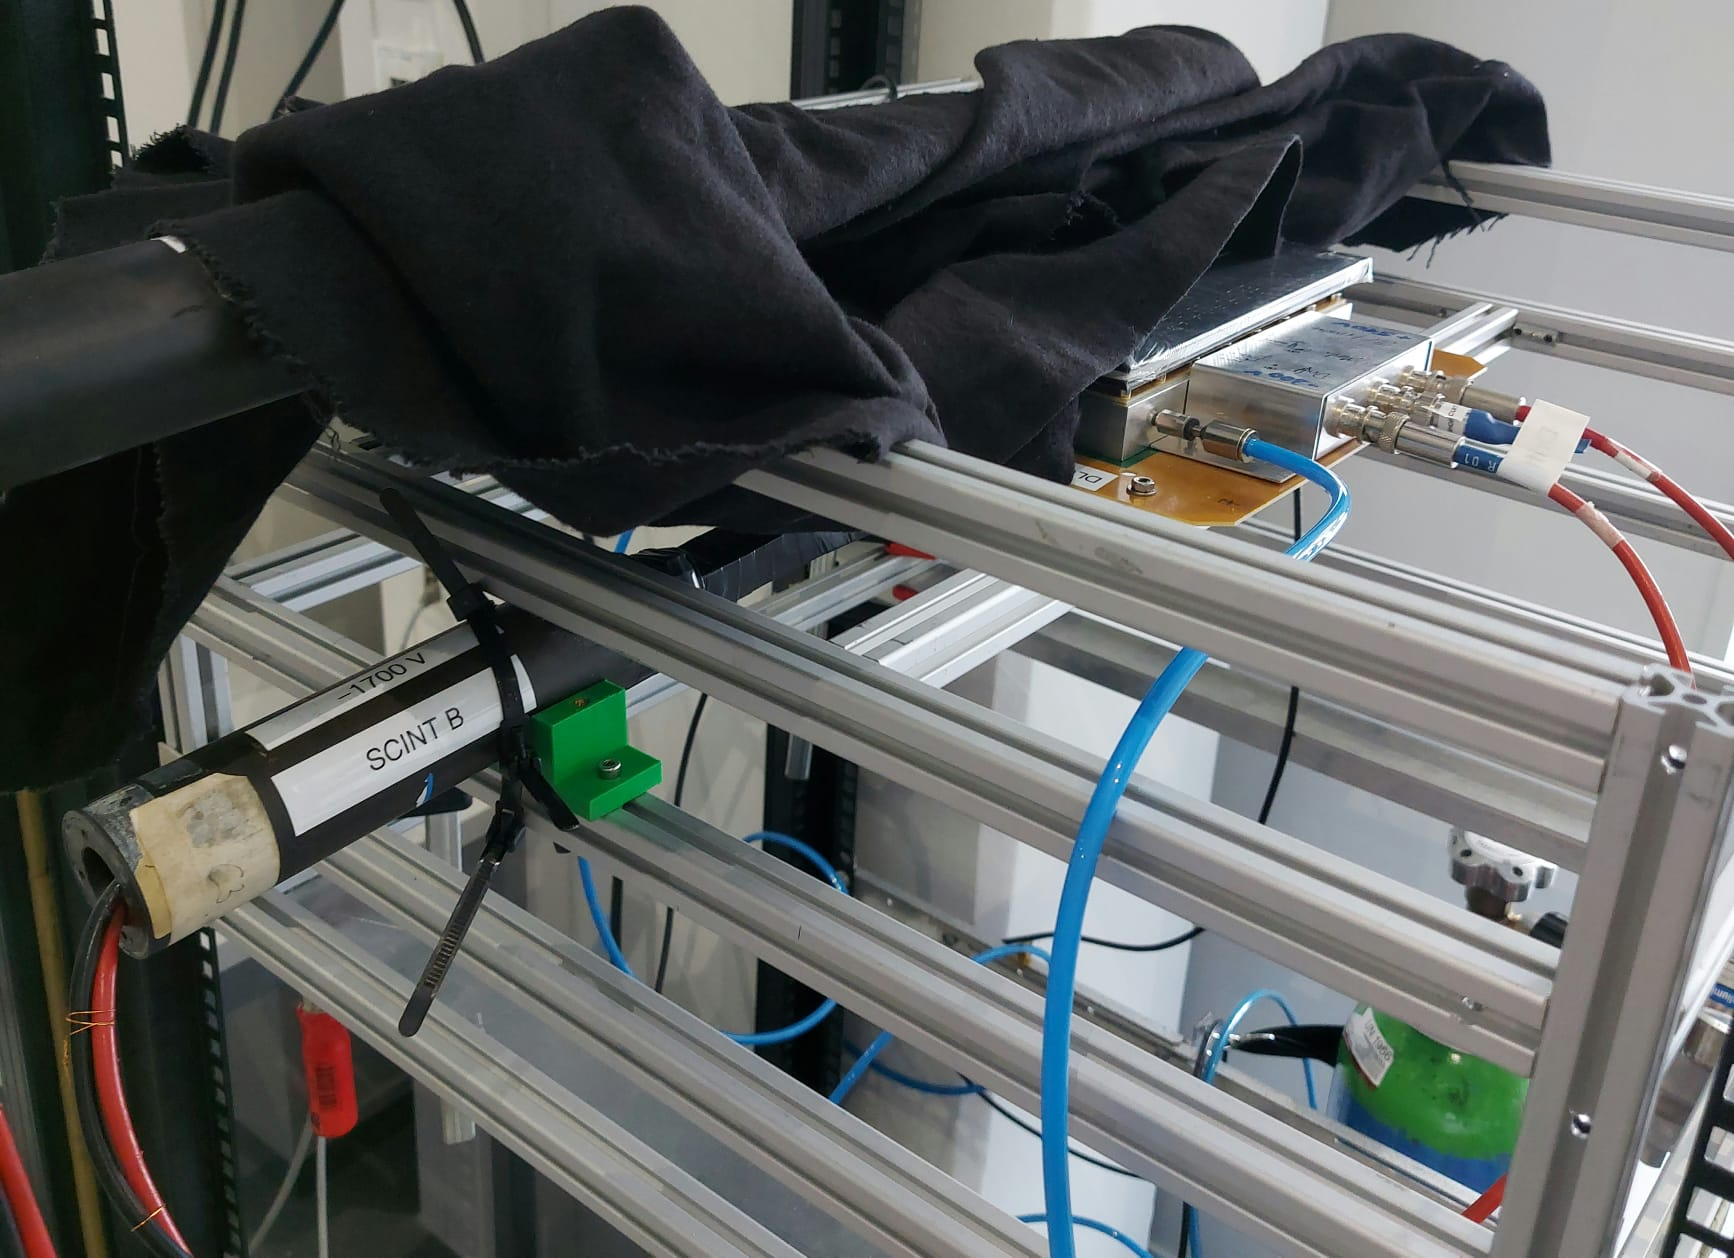
\includegraphics[width=\linewidth]{figures/setup_ROT.jpeg}
  \caption{Used setup of micromegas detector and scintillators at ROT to measure cosmic muon events.}
  \label{fig:setup_ROT}
\end{figure}

As can be seen, one of the scintillators is covered up by a cloth. 
This is because the particular scintillator did not seem to be sealed correctly and thus is covered to increase its efficiency.
The scintillators are provided with voltages of \SI{1700}{\volt} and \SI{1250}{\volt}. 
They are provided by a high voltage module \cite{Micromega} along with the voltages for the micromegas detector of \SI{-300}{\volt} and \SI{510}{\volt}.

Additionally, more modules \cite{Micromega} are used to set up the trigger logic of the detector.
The trigger logic ensures, that the detector only counts hits when both scintillators register an event so noise is minimized and only particles which pass through the detector are counted.

The readout system of the detector consists of four APVs \cite{APV}, two for each axis, and a minicrate, which are triggered by the trigger logic and then send the received data to a PC where the data readout is handled by the mmDAQ software \cite{mmDAQ}.


\subsection{Experimental Procedure}
To set up the trigger logic the scintillators are placed directly on top of each other, so events would be registered at both of them at a higher rate.
This positioning is only used for first setting up the trigger logic.
For data taking the scintillators are returned to their original positions above and below the micromegas detector.
Looking at the scintillator signal directly with an oscilloscope one could observe a signal as shown in \autoref{fig:scintillator_signal}.

\begin{figure}
  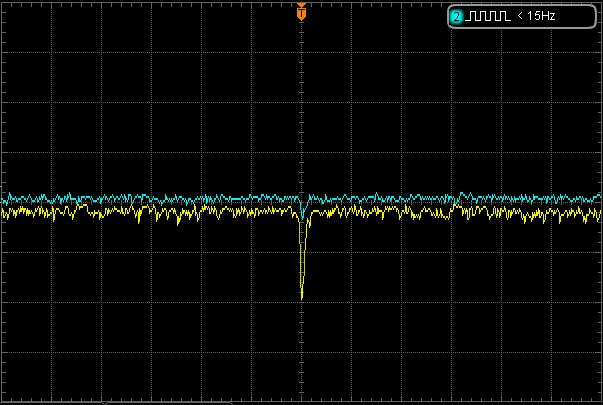
\includegraphics[width=\linewidth]{figures/DS1Z_QuickPrint5_cropped.png}
  \caption{Signal of both scintillators without modification.}
  \label{fig:scintillator_signal}
\end{figure}

The signals are quite weak, so they are amplified using the 12-channel photo-multiplier amplifier module which has a gain of 10.
After amplifying the signal it is discriminated to search for coinciding scintillator signals.
The discriminator only triggers when a certain signal threshold is reached. 
When triggered the discriminator outputs a constant signal over a given discrimination time.
By setting the threshold most of the noise is filtered.
Because the discriminator has a set discrimination time multiple events in this time will not be registered. 
For measuring cosmic muon rays this is not relevant because the events are of low frequency.

After producing the discriminated signal one wants to check for coincidence between both signals of the scintillators.
To achieve this a logic unit with an \texttt{and} operation is used on both discriminated signals.
This yields only a signal when both scintillators have overlapping discrimination signals as shown in \autoref{fig:disc_signal}.
Due to the overlap it can be assumed that both scintillator signals stem from the same particle passing though them.
When there is no overlap it is evident that the scintillators are hit by different particles and there is no trigger signal.
At last the registered events are counted with a simple counter module to check if the trigger is registering events at a realistic rate.

\begin{figure}
  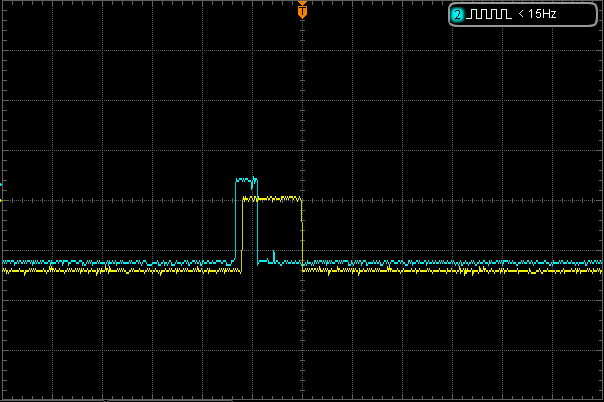
\includegraphics[width=\linewidth]{figures/DS1Z_QuickPrint2_cropped.png}
  \caption{Discriminated signal of one scintillator (yellow) and trigger signal after logic unit (blue).}
  \label{fig:disc_signal}
\end{figure}

After setting up the trigger logic data can be taken. 
First a pedestal run is necessary to configure the readout electronics, then over a time of roughly \SI{60}{\minute} cosmic muon rays are captured.
Extracting the information from the \texttt{.root} file yields the hitmap in \autoref{fig:muon_hitmap}.

\begin{figure}
  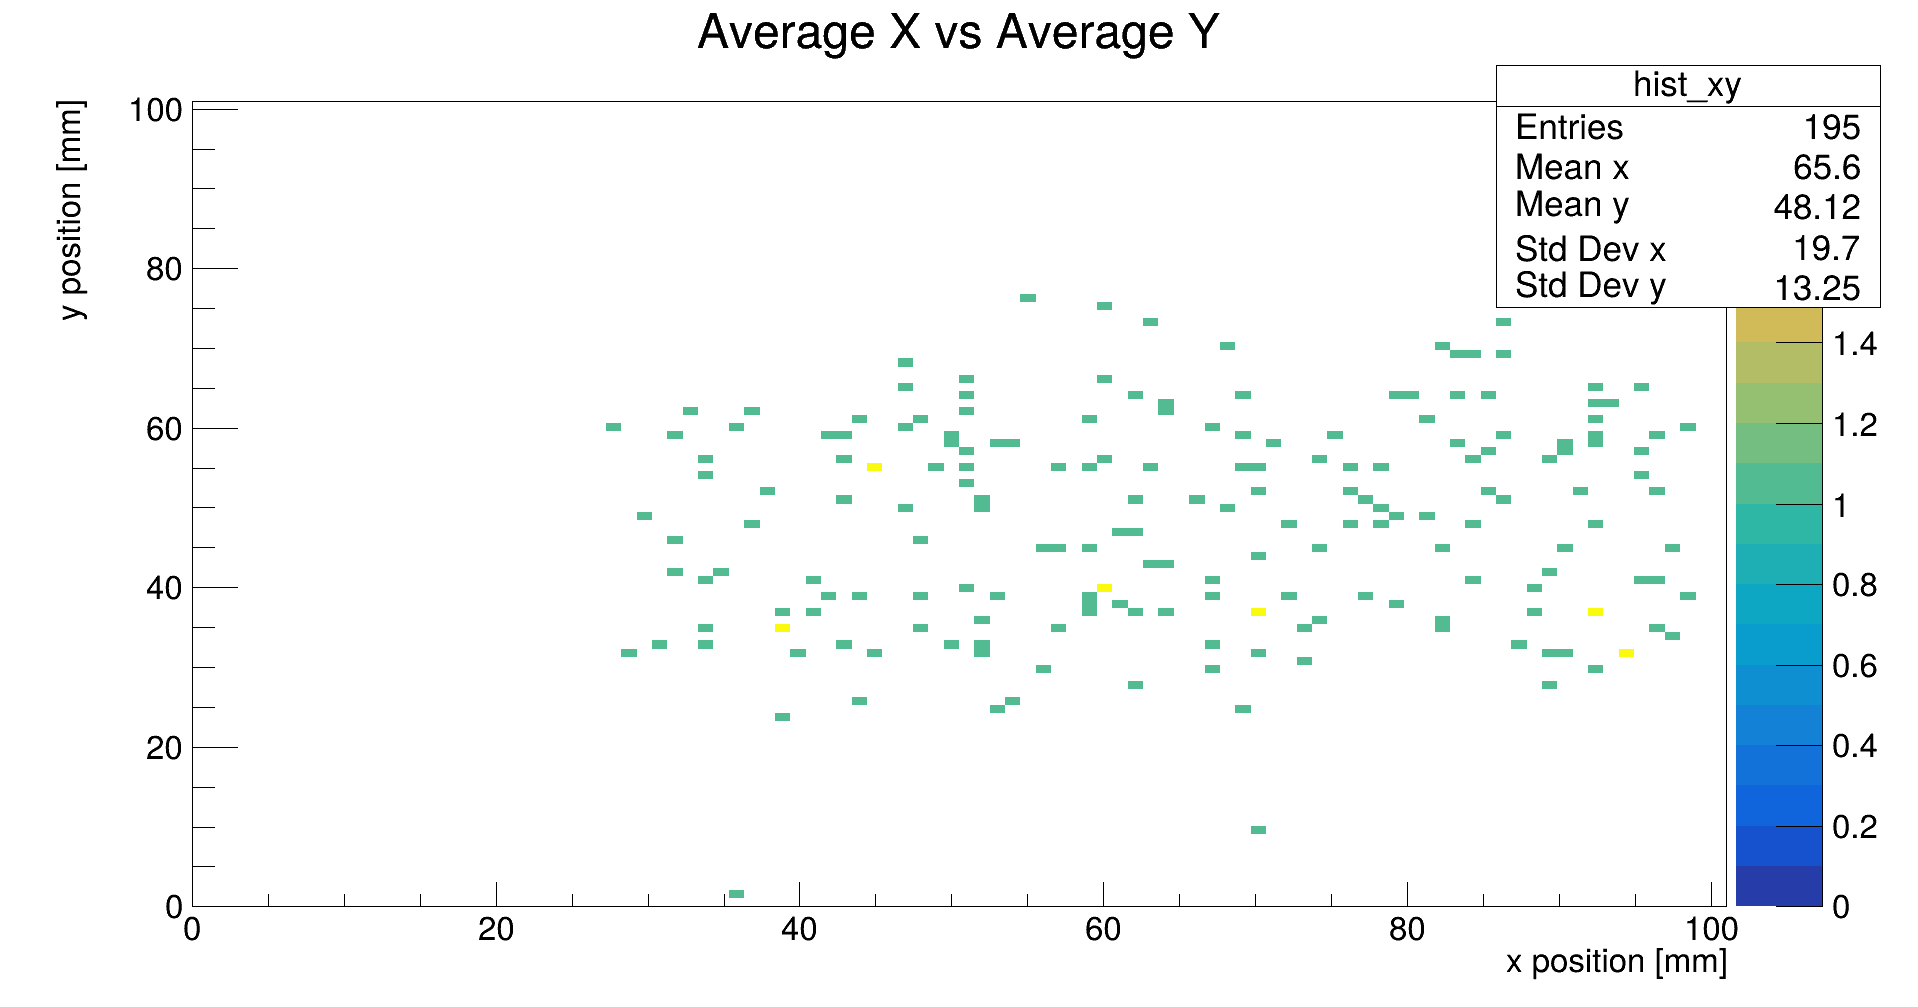
\includegraphics[width=\linewidth]{../src/elsa/finished_plots/muon_hitmap_avg.png}
  \caption{Averaged hitmap of cosmic muons.}
  \label{fig:muon_hitmap}
\end{figure}

% As can be seen our scintillators were orientated parallel to each other and overlapped along their whole length.
% Because of our trigger logic we only register events at places where our scintillators overlap. 
% It is clear that other events may have happened but were not read out because our trigger logic did not register overlapping scintillator signals.
% The muons seem to be evenly distributed over the area of the scintillators which seems logical, because cosmic radiation should be homogeneously distributed.
% We can also see some events which are not in the area of our scintillators. 
% Those can either be explained by noise or other interferences in the data taking process.
% It can also be possible that the detector readout was triggered by an event in the area of the scintillators while another event happened at a different place in the detector.
% Because one event triggered the detector readout another event which happened may have been read out as well.

As can can be seen events occur only in the area where the scintillators overlap, resulting in a rectangular shape.
This is explained by the trigger logic, which only triggers detector readout when a particle passes through both scintillators.
Some events are observed outside of the area covered by the scintillators, which can be explained by two particles simultaneously hitting the detector, where one triggers the readout.
Aside from another particle detector noise may be captured.
Over a time of roughly \SI{60}{\minute} 195 events are captured, which is equivalent to a rate of \SI{3.25}{\text{µ}\per\minute}.
Muons arrive at sea level with an average flux of \SI{1}{\text{µ}\per\centi\meter\squared\per\min} \cite{muon}.
According to the hitmap the scintillators covered an area of approximately $\SI{7}{\centi\meter}\cdot\SI{5}{\centi\meter}=\SI{35}{\centi\meter\squared}$, which should correspond to a count of 2100 events after \SI{60}{\min}.
The reduced amount of registered events is explained by muons coming at an angle and thus not triggering the readout system.
Another explanation is the location at which the experiment is set up. 
The detector is placed in the basement below the ROT building. 
Therefore some muons are already absorbed by passing through the building and the rate of detected muons is lowered.
With these considerations the measured rate of \SI{3.25}{\text{µ}\per\min} over an area of \SI{35}{\centi\meter\squared} or \SI{0.09}{\text{µ}\per\centi\meter\squared\per\min} is realistic.
The measured rate is one order of magnitude smaller than the average muon flux at sea level \cite{muonsea} which is justified by the mentioned circumstances. 

%-----------------------------------------------------------------------------------------------------------------------------

\section{Multiple Scattering}
\subsection{Experimental Setup}
To observe multiple scattering, an electron beam of $\SI{2.9}{GeV}$ is provided by the stretcher ring of ELSA \cite{ELSA}, whose beam exit is shown in \autoref{fig:beam_setup_elsa}. 
The setup of the micromegas detector with the scintillators and the trigger logic, used and tested with the cosmic data, is placed a few metres in front of the output of the accelerator, such that the beam hits the detector as seen in \autoref{fig:detector_setup_elsa}. 
This is ensured by a laser, build in at the end of the accelerator, which could be slid into the middle of the opening to point along the beam line. 
However, it is known that the laser points a few centimetres lower than the actual beam. 
This must be considered while placing the targets.
A metal bar is mounted close to the detector thus the targets can be placed in a distance between $\SI{5.5\pm 0.5}{cm}$ and $\SI{105.5\pm 0.5}{cm}$ to the first scintillator into the beam, where the uncertainties come from the measuring tape used to evaluate these distances. 
The laser is used to adjust the bar and to ensure a free beam path up to the detector or the placed material.
The available materials with their thicknesses are listed in \autoref{tab:available_materials}. 
These were measured by a previous group with a caliper, so uncertainties of $\SI{0.1}{mm}$ are assumed, which is roughly checked with the maesuring tape.


\begin{table}\centering
  \renewcommand*{\arraystretch}{1.1}
  \begin{tabular}{c|c||c|c}
    \multicolumn{2}{c||}{aluminium} & \multicolumn{2}{c}{Copper} \\
    {\fontsize{8}{3}\selectfont $x_i/\si{cm}$} & {\fontsize{8}{3}\selectfont \#} & {\fontsize{8}{3}\selectfont $x_i/\si{cm}$} & {\fontsize{8}{3}\selectfont \# } \\\hline \rule{0pt}{3ex}
    \num{1.22\pm 0.01} & 2 & \num{0.2\pm 0.01} & 3 \\
    \num{2.5\pm 0.01} & 1 & \num{0.5\pm 0.01} & 2 \\
    \num{5\pm 0.01} & 1 & \num{1.48\pm 0.01} & 2 \\
    \num{9.96\pm 0.01} & 1 & & \\
    \num{9.93\pm 0.01} & 1 & & \\
  \end{tabular}\vspace{3mm}
  \caption{Available scattering materials of thickness $x_i$ and quantity $\#$.}
  \label{tab:available_materials}
\end{table}

\begin{figure}
  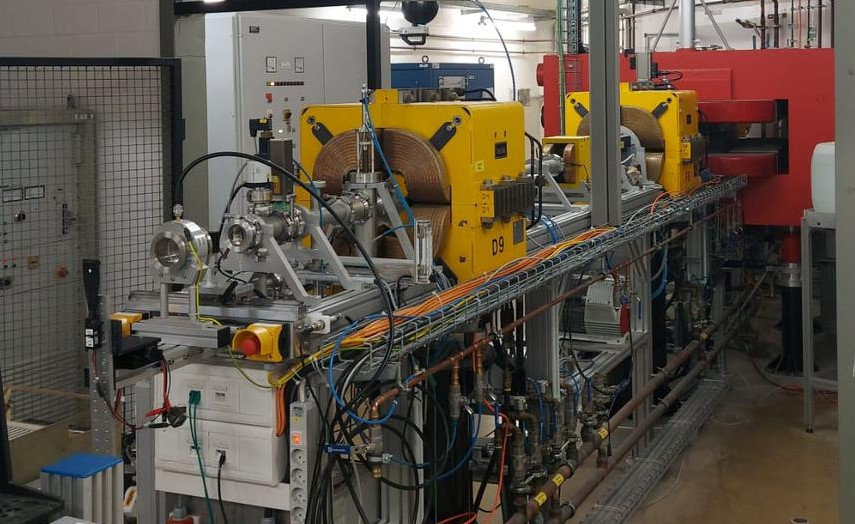
\includegraphics[width=\linewidth]{figures/beam_setup_elsa.jpg}
  \caption{Exit of ELSA.}
  \label{fig:beam_setup_elsa}
\end{figure}

\begin{figure}
  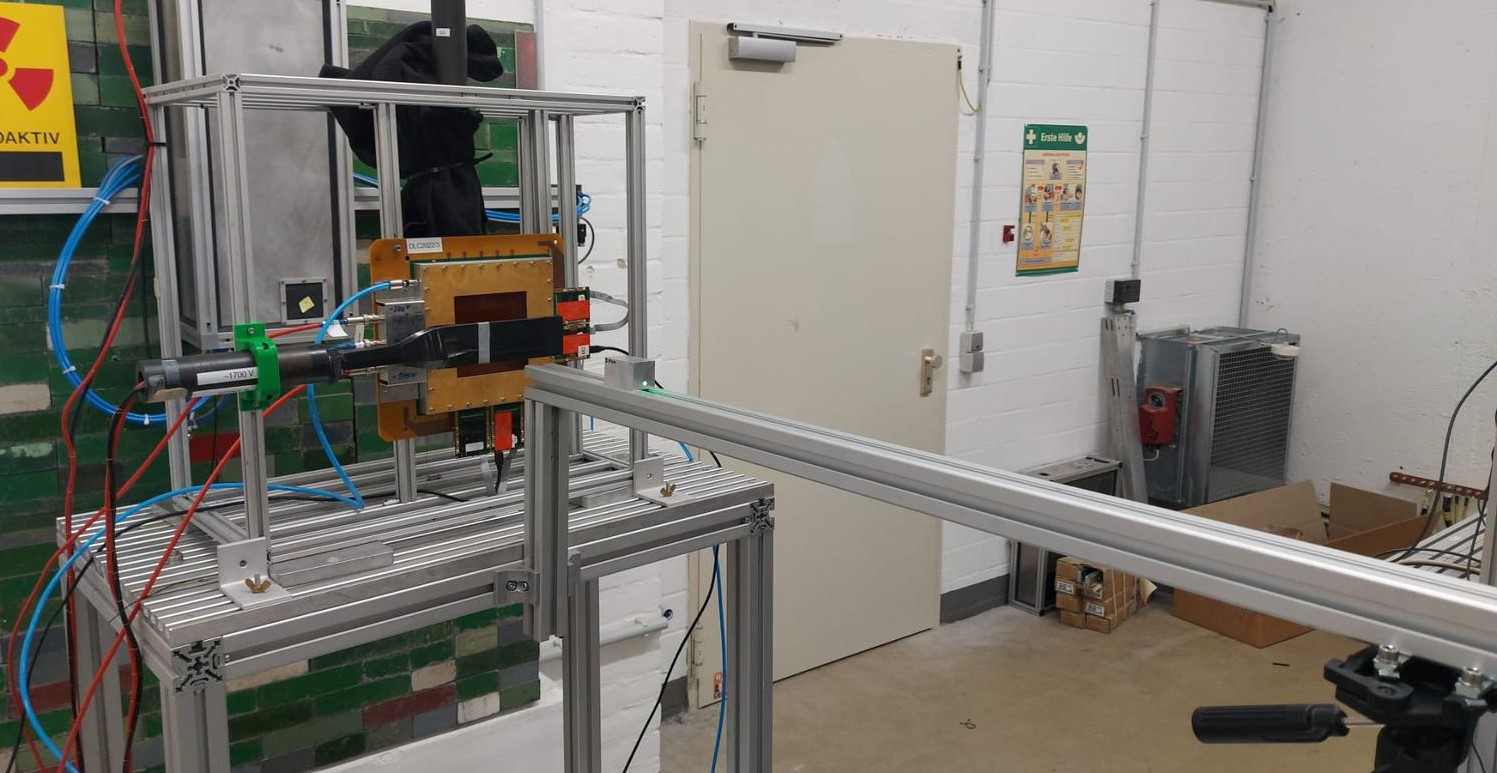
\includegraphics[width=\linewidth]{figures/detector_setup_elsa.jpg}
  \caption{Setup of the detector and the metal bar, to place the targets on it and align them with the laser.}
  \label{fig:detector_setup_elsa}
\end{figure}

\subsection{Experimental Procedure}
After controlling the setup of the detector including the trigger logic and the right adjustment of the metal bar, a test run without any target in the beam is performed, to ensure the functionality of the setup and the data taking program.
Afterwards, multiple runs are recorded for both materials.
The thicknesses $x$ of the targets are changed by placing different blocks of one material in a row. 
$x$ is always chosen to be approximately multiples $m$ of the radiation length $X_0$ \cite{radlength} of the material, with $m\in\{0.5,1,2,3\}$. 
The distance $d$ between the scintillator and the leading edge of the material is always $d=\SI{40\pm0.5}{cm}$.
To include the distance from the scintillator to the middle of the drift chamber in the detector, an additional spacing of $\SI{5\pm2}{cm}$ is assumed, leading to an overall distance of $d'=\SI{45\pm2}{cm}$.
In total eight runs, one for each $m$ and both materials, are recorded. 
The exact configurations for the different measurements are listed in \autoref{tab:config_materials}.

\begin{table}\centering
  \renewcommand*{\arraystretch}{1.15}
  \begin{tabular}{c|c|c}
    & aluminium & copper \\
    & {\fontsize{7}{5}\selectfont ($X_0=\SI{8.897}{cm}$)} & {\fontsize{7}{5}\selectfont ($X_0=\SI{1.436}{cm}$)} \\\hline
    $m$ & $\sum x_i/cm = x /cm$ & $\sum x_i/cm = x /cm$ \\\hline\hline\rule{0pt}{6ex}
    $0.5$ & \num{5\pm 0.01} & $\begin{array}{r}
                \num{0.5\pm 0.01} \\
                +\,\num{0.2\pm 0.01} \\\hline
                =\,\num{0.7\pm 0.01}    
              \end{array}$ \\\hline
    $1$ & \num{9.93\pm 0.01} & \num{1.48\pm 0.01} \\\hline
    $2$ & $\begin{array}{r}
      \num{1.22\pm 0.01} \\
      +\,\num{2.5\pm 0.01} \\
      +\,\num{5\pm 0.01} \\
      +\,\num{9.93\pm 0.01} \\\hline
      =\,\num{18.65\pm 0.02}
    \end{array}$ & $\begin{array}{r}
                      2\times\num{1.48\pm 0.01} \\\hline
                      =\,\num{2.96\pm 0.01}
                    \end{array}$ \\\hline
    $3$ & $\begin{array}{r}
      \num{2.5\pm 0.01} \\
      +\,\num{5\pm 0.01} \\
      +\,\num{9.93\pm 0.01} \\
      +\,\num{9.96\pm 0.01} \\\hline
      =\,\num{27.39\pm 0.02}
    \end{array}$ & $\begin{array}{r}
                      2\times\num{0.2\pm 0.01} \\
                      +\,2\times\num{0.5\pm 0.01} \\
                      +\,2\times\num{1.48\pm 0.01} \\\hline
                      =\,\num{4.36\pm 0.02}
                    \end{array}$ \\\hline
  \end{tabular}\vspace{3mm}
  \caption{Specific configurations of used materials with radiation length $X_0$ and overall thicknesses $D$ for different multiples $m$ of $X_0$.}
  \label{tab:config_materials}
\end{table}

\subsection{Data Analysis}
The recorded data of the run without scattering material in the beam is shown as a hitmap in \autoref{fig:hitmap_notarget}. 
\begin{figure}
  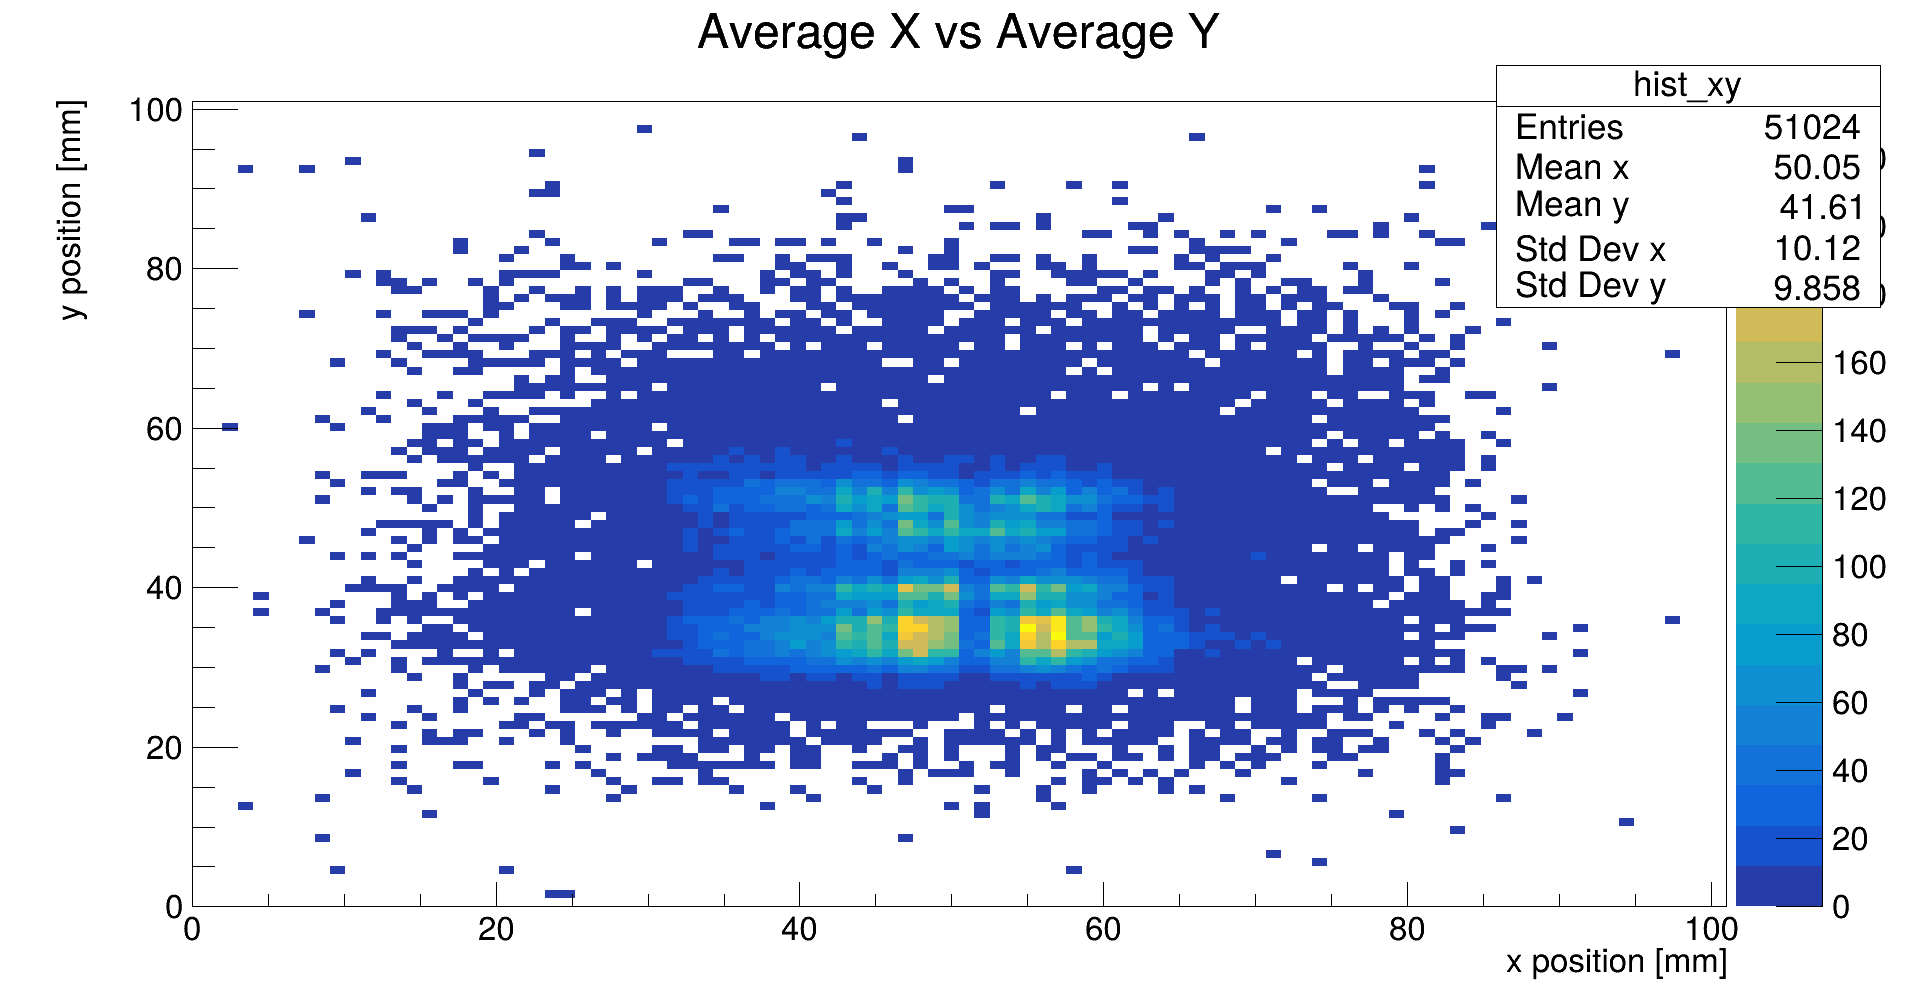
\includegraphics[width=0.9\linewidth]{../src/elsa/finished_plots/xy_hitmap_0.png}
  \caption{Hitmap for the electron beam on the detector without scattering material.}
  \label{fig:hitmap_notarget}
\end{figure}
The distribution of the electrons in the x-direction is wider as in y-direction, resulting in an oval-shaped beam.
To analyse the influence of a material in order to observe multiple scattering effects, a narrower beam width is advantageous, as the additional broadening due to scattering becomes more distinguishable.
Moreover, \autoref{fig:x_hist_notarget} shows, that one APV of the detector positioned in x-direction contains multiple defect stips in the region of interest.
Therefore, in the following analysis, only the y-direction is considered. The counted events whithout scattering material are shown in \autoref{fig:y_hist_notarget}.

\begin{figure}
  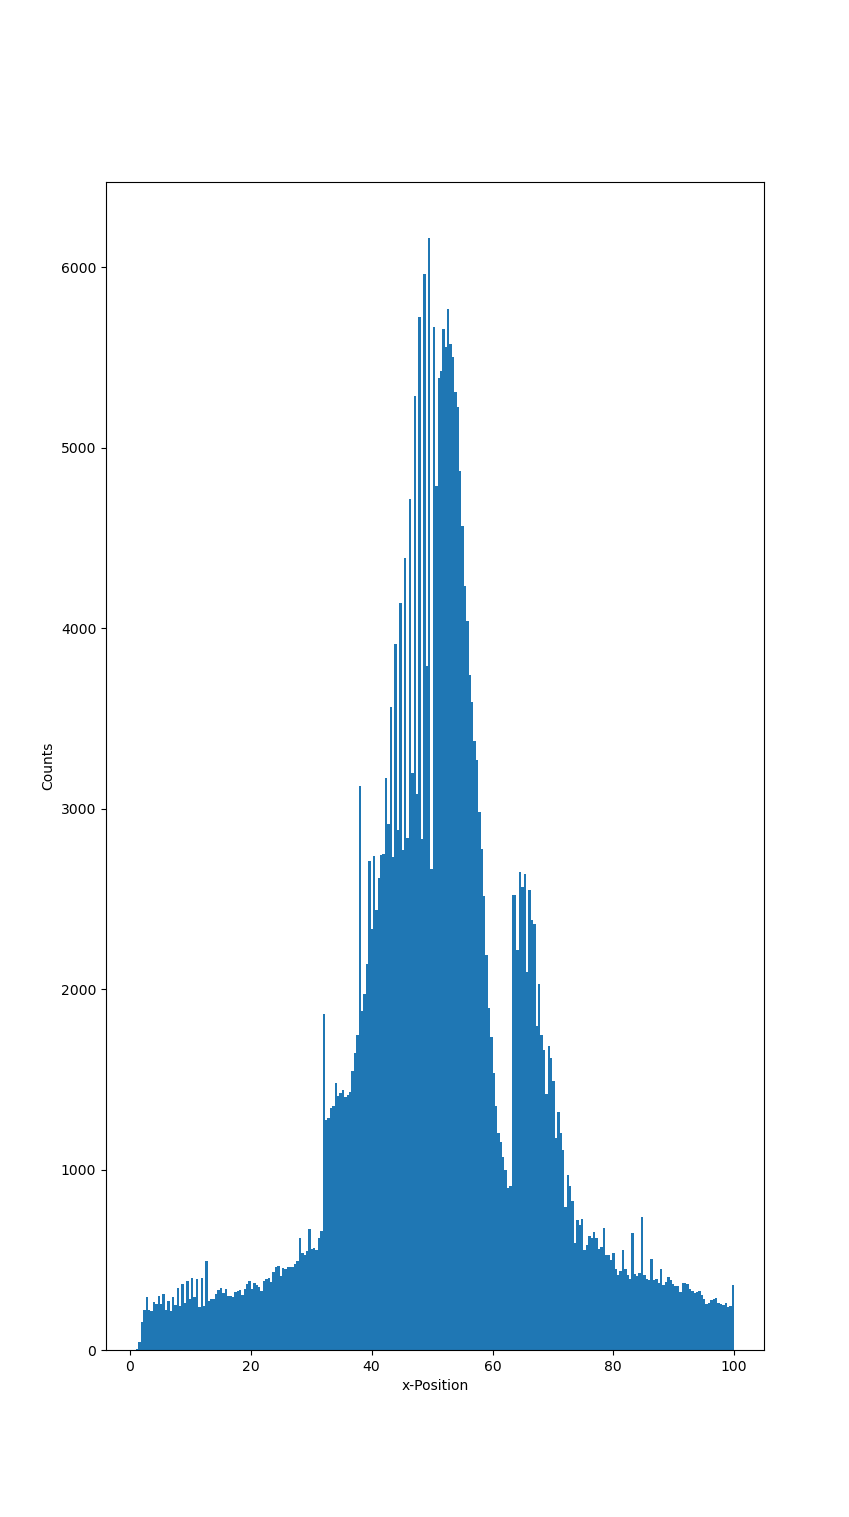
\includegraphics[width=0.9\linewidth]{../src/elsa/finished_plots/UnfilteredNoMaterialX.png}
  \caption{Counted hits in x-direction without scattering material.}
  \label{fig:x_hist_notarget}
\end{figure}

\begin{figure}
  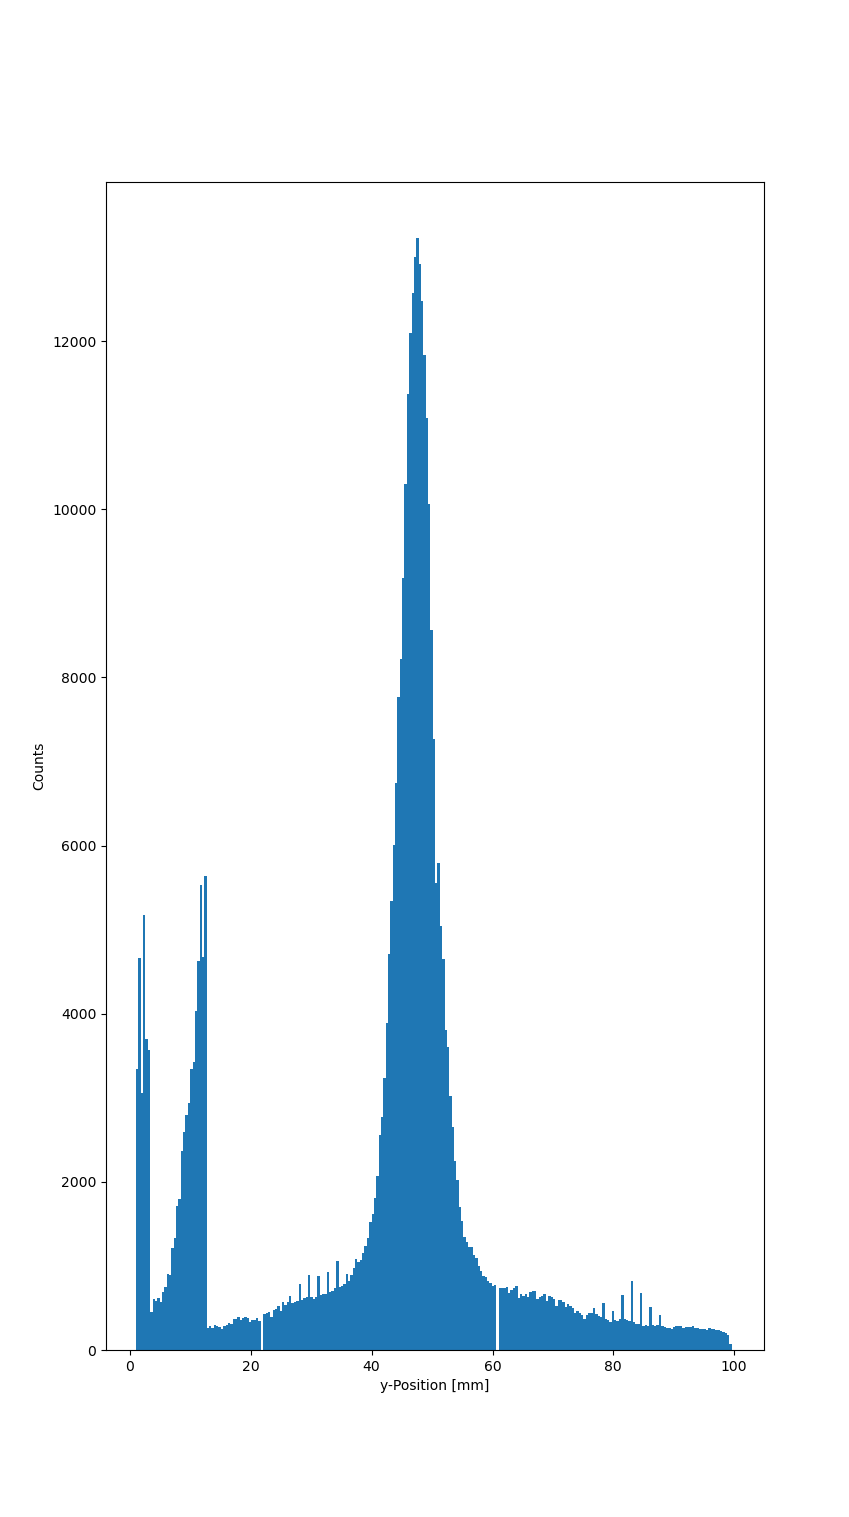
\includegraphics[width=0.9\linewidth]{../src/elsa/finished_plots/unfiltered_noMaterial.png}
  \caption{Counted hits in y-direction without scattering material.}
  \label{fig:y_hist_notarget}
\end{figure}

Both the distribution in x and in y direction contain, additionally to the gaussian curve, other peaks in the foothills of the distribution, which is also observed for all recorded runs.
By cutting away events of large charge deposition, these artifacts disappear. 
A possible reason is that the detector is more sensitive at these strips which leads to more counted events.
Additionally one observes, that at one specific point i.e.\ one specific strip in the detector, no event seems to be counted.
This is due to the way the strips are converted to millimetre.
To do this, one has to multiply the strip by the length of the detector (in the corresponding direction) and divide by the number of strips.
This will lead to rounding issues, where it is possible that one millimetre is left out, because a bin can only be of type integer.

In general, the number of events increase gaussian from lower to higher y-positions before suddenly falling close after the maximum and start decreasing again gaussian. 
This behaviour is observed for every run though with different intensity. 
Because the sharp edge is localized exactly in the middle of the detector, it is evidently caused by a different behaviour of the two APVs, used for the readout of one direction. 
Apparently, one has a higher charge sensitivity so its probability to count events is higher than the other, which results in an asymmetrical image. 

In order to evaluate the effects of multiple scattering, a gaussian distribution is fittet to the data. 
This is done by fitting only to one side of the curve due to the asymmetry, which can be seen for aluminium as the scattering target with a thickness of approximately two times the radiation length in \autoref{fig:2alu} and collected for all runs in \autoref{fig:alu_gaus}.

\begin{figure}
  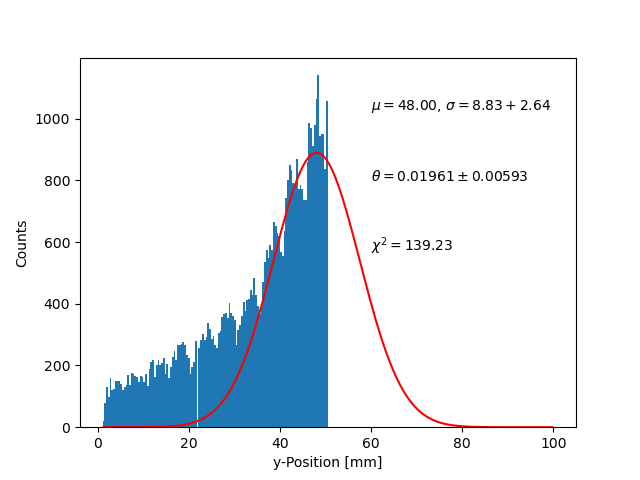
\includegraphics[width=0.9\linewidth]{../src/elsa/finished_plots/Aluminium, Two Radiation Lengths, 40cm Distance.png}
  \caption{Counted hits for aluminium with $x\approx2\cdot X_0$.}
  \label{fig:2alu}
\end{figure}

It is noticeable, that in a very regularly pattern the gaussian distribution contains dips in the event counter. (Begründung)
%The distance between two dips is $\SI{5}{mm}$, which matches exactly the height of one rectangle of the grid structure in the detector described in \autoref{subsec:detector_specific}. This indicates the possible reason for the dips, that every $n$-th strip in one rectangle has a lower sensitivity than the others, leading to the observed effect.

To calculate the RMS of the deflection angle $\theta_\text{exp}$, the standard deviation $\sigma_\text{mat}$ of the curves, available through the parameters of the fit, is used. To consider the width of the electron distribution without any scattering, it is replaced by the modified standard deviation
\begin{equation} \label{eq:sigma_mod}
  \sigma = \sqrt{\sigma_\text{mat}^2 - \sigma_\text{0}^2},
\end{equation}
where $\sigma_\text{0}$ is the standard deviation of the distribution without any scattering material in the beam shown in \autoref{fis:hist_notarget}. 
Via \autoref{eq:theta_exp} this leads to the experimental value.

\begin{figure}
  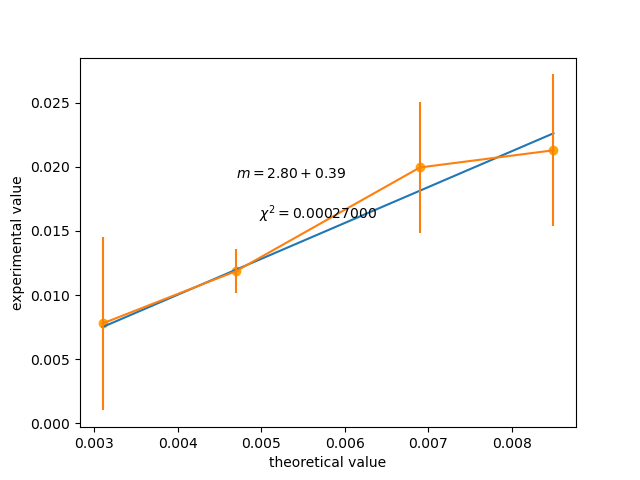
\includegraphics[width=0.9\linewidth]{../src/elsa/finished_plots/Copper.png}
  \caption{Correlation between experimental and theoreticle RMS scattering angle of copper.}
  \label{fig:correlation_cop}  
\end{figure}

\begin{figure}
  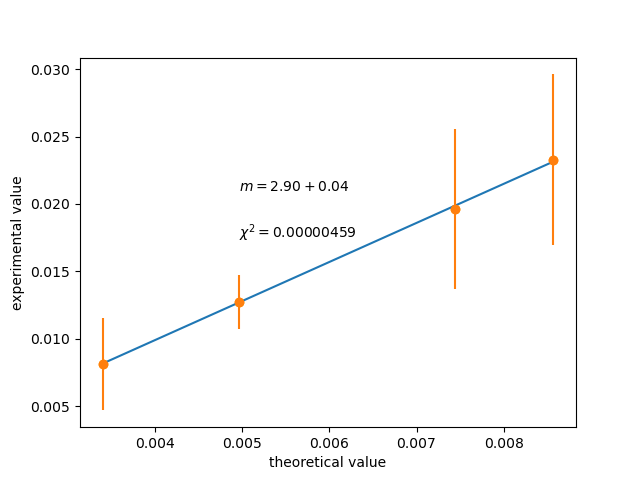
\includegraphics[width=0.9\linewidth]{../src/elsa/finished_plots/Aluminium.png}
  \caption{Correlation between experimental and theoreticle RMS scattering angle of aluminium.}
  \label{fig:correlation_alu}  
\end{figure}


\begin{table}
  \begin{tabular}{ccc}
    \toprule
    $\tfrac{x}{X_0}$ & $\theta _\text{exp}$/rad & $\theta _\text{theo}$/rad \\
    \midrule
    1/2 & \num{.00812+-.00343}[42\%,1.3$\sigma$] & 0.0343\\
    1 & \num{.01274+-.00198}[16\%,3.9$\sigma$] & 0.00497\\
    2 & \num{.01961+-.00593}[30\%,2$\sigma$] & 0.00744\\
    3 & \num{.02329+-.00632}[27\%,2.3$\sigma$] & 0.0858\\
    \midrule
    1/2 & \num{.00778+-.00678}[87\%,0.7$\sigma$] & 0.00318\\
    1 & \num{.01187+-.00171}[14\%,4.2$\sigma$] & 0.00476\\
    2 & \num{.01995+-.00510}[26\%,2.6$\sigma$] & 0.00692\\
    3 & \num{.02129+-.00592}[28\%,2.2$\sigma$] & 0.00851\\
    \bottomrule
  \end{tabular}
  \caption{An overview of the experimentally and theoretically calculated angles; aluminium top and copper bottom. 
  The relative error and standard deviation from the theoretical values is given in the square brackets.}
\end{table}
To compare this experimental result with the theoretical discription, $\theta_\text{exp}$ is plotted against $\theta_\text{theo} = \theta_0$ evaluated via \autoref{eq:Highland}, as shown for copper in \autoref{fig:correlation_cop} and aluminium in \autoref{fig:correlation_alu}.
Note that the following discussion can be applied to both.

The relative error for the deflection angle of $\tfrac{x}{X_0}=1/2$ is very large compared to the other thicknesses, for both aluminium and copper.
This is due to the overall broad shape of the data compared to the small width making the fit unprecise.
The resulting deviation is thus small and close to one sigma, but only due to the large relative error.

For $\tfrac{x}{X_0}=1$ the relative error is closer to 10\% making these values more reliable for a measurement to be compared to the theory.
In comparison with the other measurements, the curve has the most accurate gaussian profile which is consistent with the results.
Although due to the small error the deviation is about 4 sigma and thus too far from the theoretical value to be consistent with it.

For $\tfrac{x}{X_0} \in \left\{2,3\right\}$ the relative error stays the same of about 30\% with a similar standard deviation of 2.2 sigma.
These values are the most consistent experimental values but with such a deviation also not compatible with the theory.


(To beeee or not to beeeee)

When plotting $\theta _\text{exp}$ against $\theta _\text{theo}$ one can see a clear linear relation between these two quantities.
The slope of the straight is $m_\text{Cu}=3$ and $m_\text{Al}=3$ (TODO GENAUER WERT).

$\chi ^2_\text{Cu}=TODO$ and $\chi ^2_\text{Al}=TODO$ which is ...
1)... close enough to one for it to be a good fit, thus modelling the data well.
2)... too small for an appropriate fit, thus unable to model the data in a predictive manner.

There is a systematic error for all data, which results in all angles to be three times larger than $\theta _\text{theo}$.
This can have numerous sources, some of which are discussed now.


On the continuous side of the gaussian distribution, another little unevenness is observed, as seen in (???).
It could be the continuation of the gaussian curve after the sharp edge, so instead of the assumed differences in sensitive beween the two APV's, in the middle of the distribution one counts too many events. (Begründung)

Another unwanted effect are created $\delta$-electrons, which also could hit the detector and lead to multiple hits for one event i.e. one readout.
Moreover, the possibility of inelastic scattering of the beam electrons in the air, leading to electromagnetic or hadronic showers, exists.
This also results in multiple hits for one event.


%-----------------------------------------------------------------------------------------------------------------------------

\section{Summary}
At ROT the measurements of the spare micromegas are taken while it is disassembled.
The captured data of the cosmic muons leads to a muon flux of approximately \SI{.09}{\text{µ}\per\centi\meter\squared\per\min} which is by a factor 10 smaller than the value from literature.
This value is explained by the absorption of muons while passing through the building, as well as muons coming at an angle and thus not being detected.

%-----------------------------------------------------------------------------------------------------------------------------

\clearpage\appendix\onecolumn


\section{Disassembled Micromegas Detector}
\renewcommand{\thefigure}{\Alph{section}\arabic{figure}}
\setcounter{figure}{0}
\renewcommand{\thetable}{\Alph{section}\arabic{table}}
\setcounter{table}{0}


\begin{figure}[h]
  \centering
    \begin{subfigure}{0.47\textwidth}
        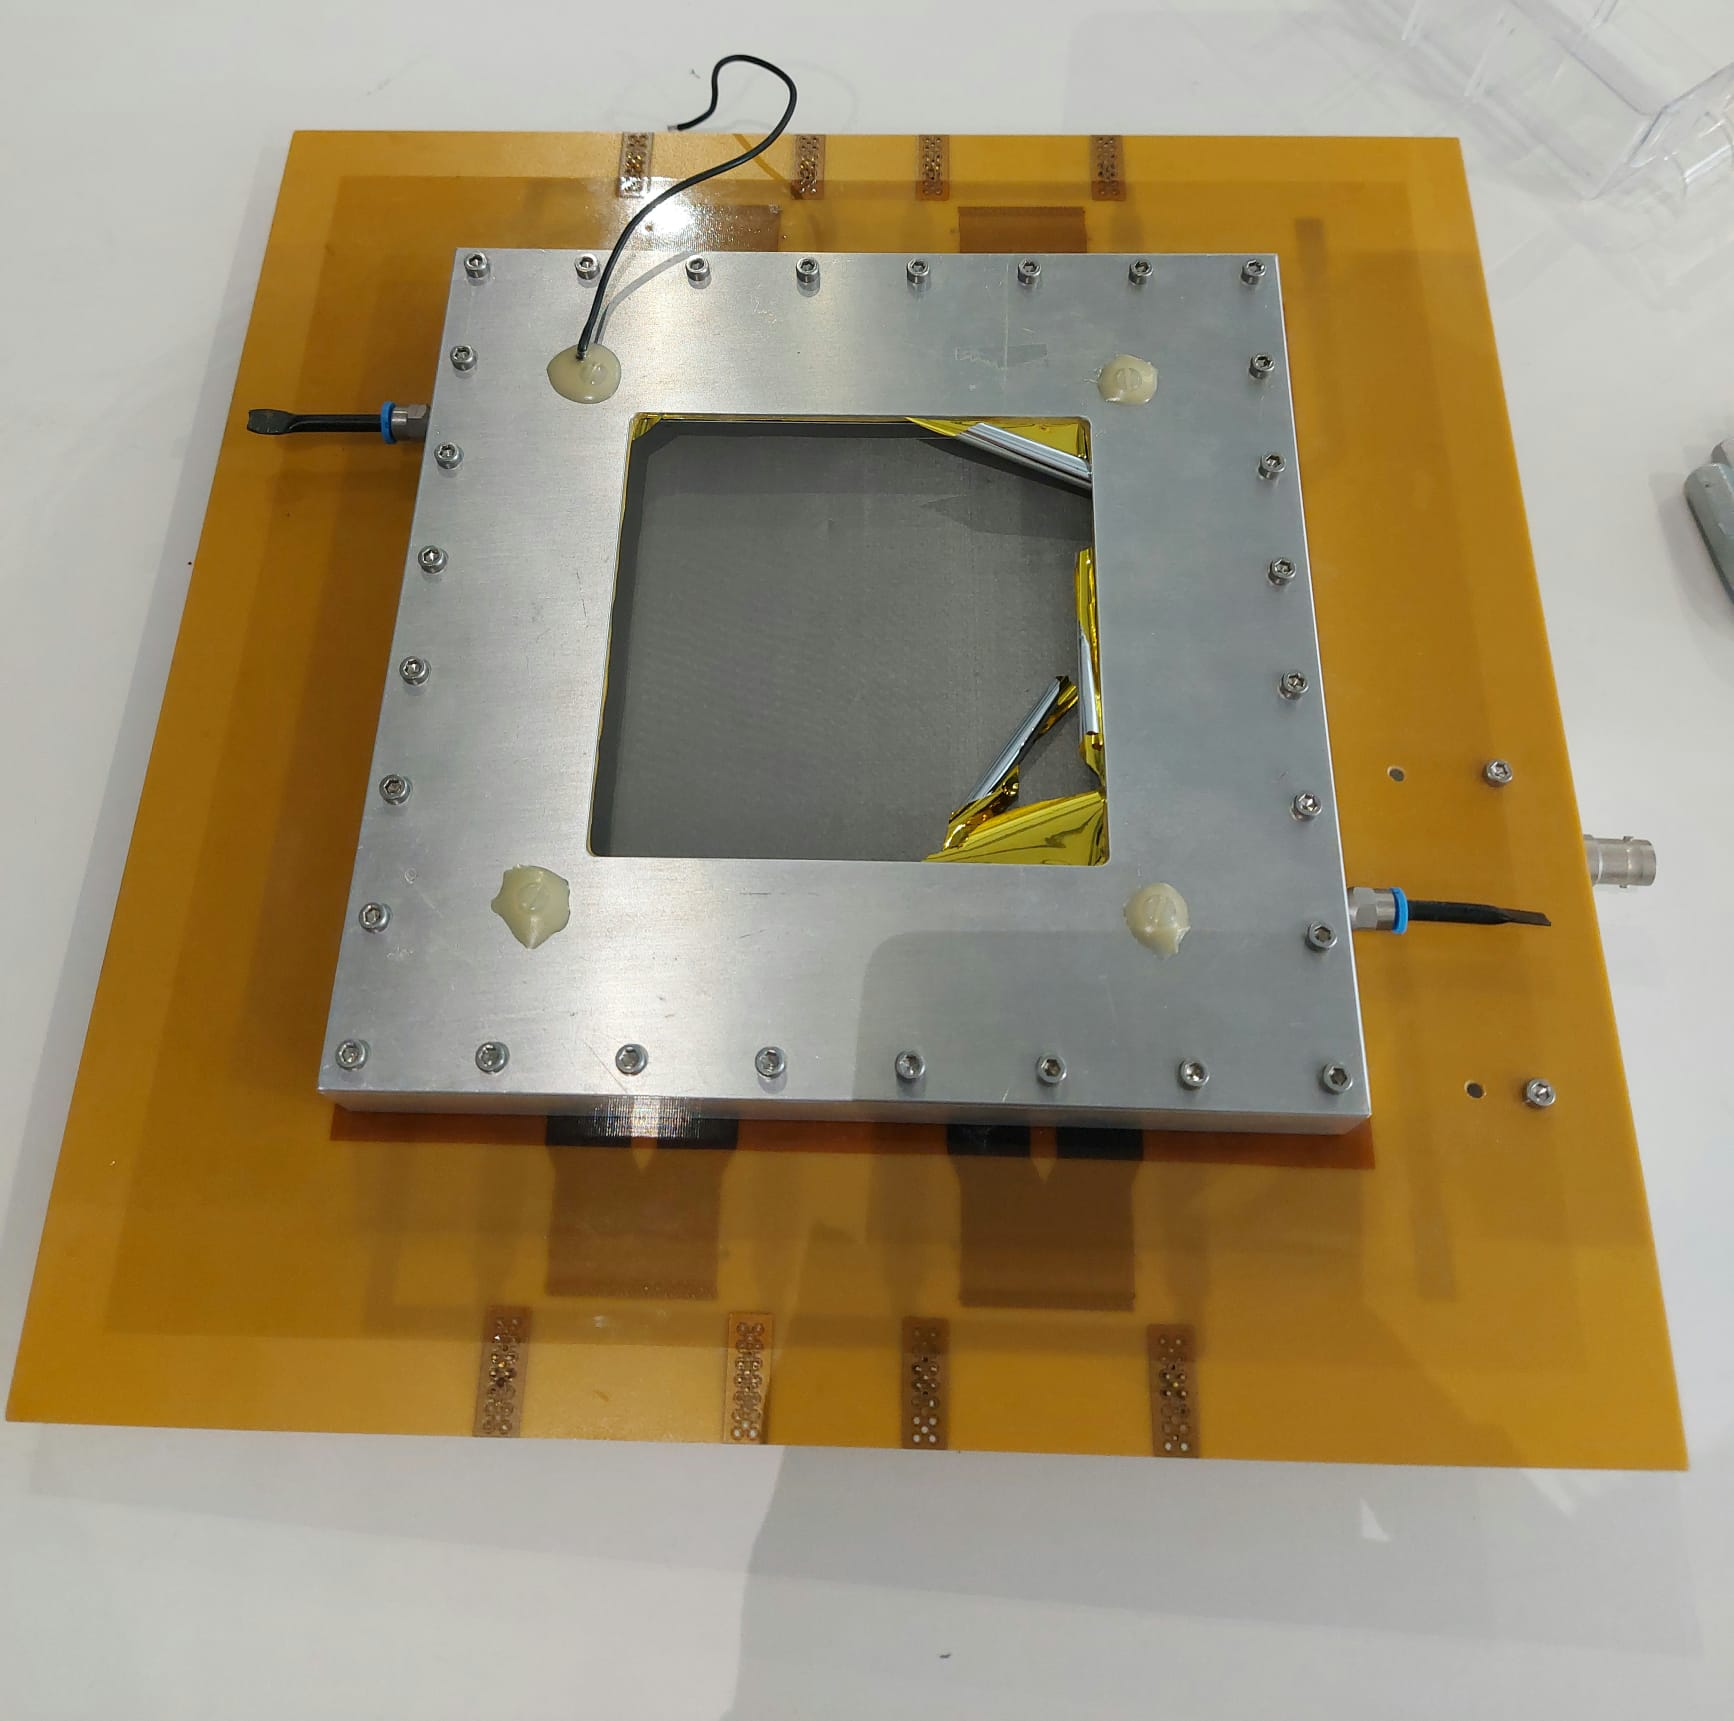
\includegraphics[width=\linewidth]{figures/micromegas_closed.jpeg}
        \caption{Front of the spare micromegas detector.}
        \label{fig:micromegas_closed}
    \end{subfigure}
    \begin{subfigure}{0.51\textwidth}
        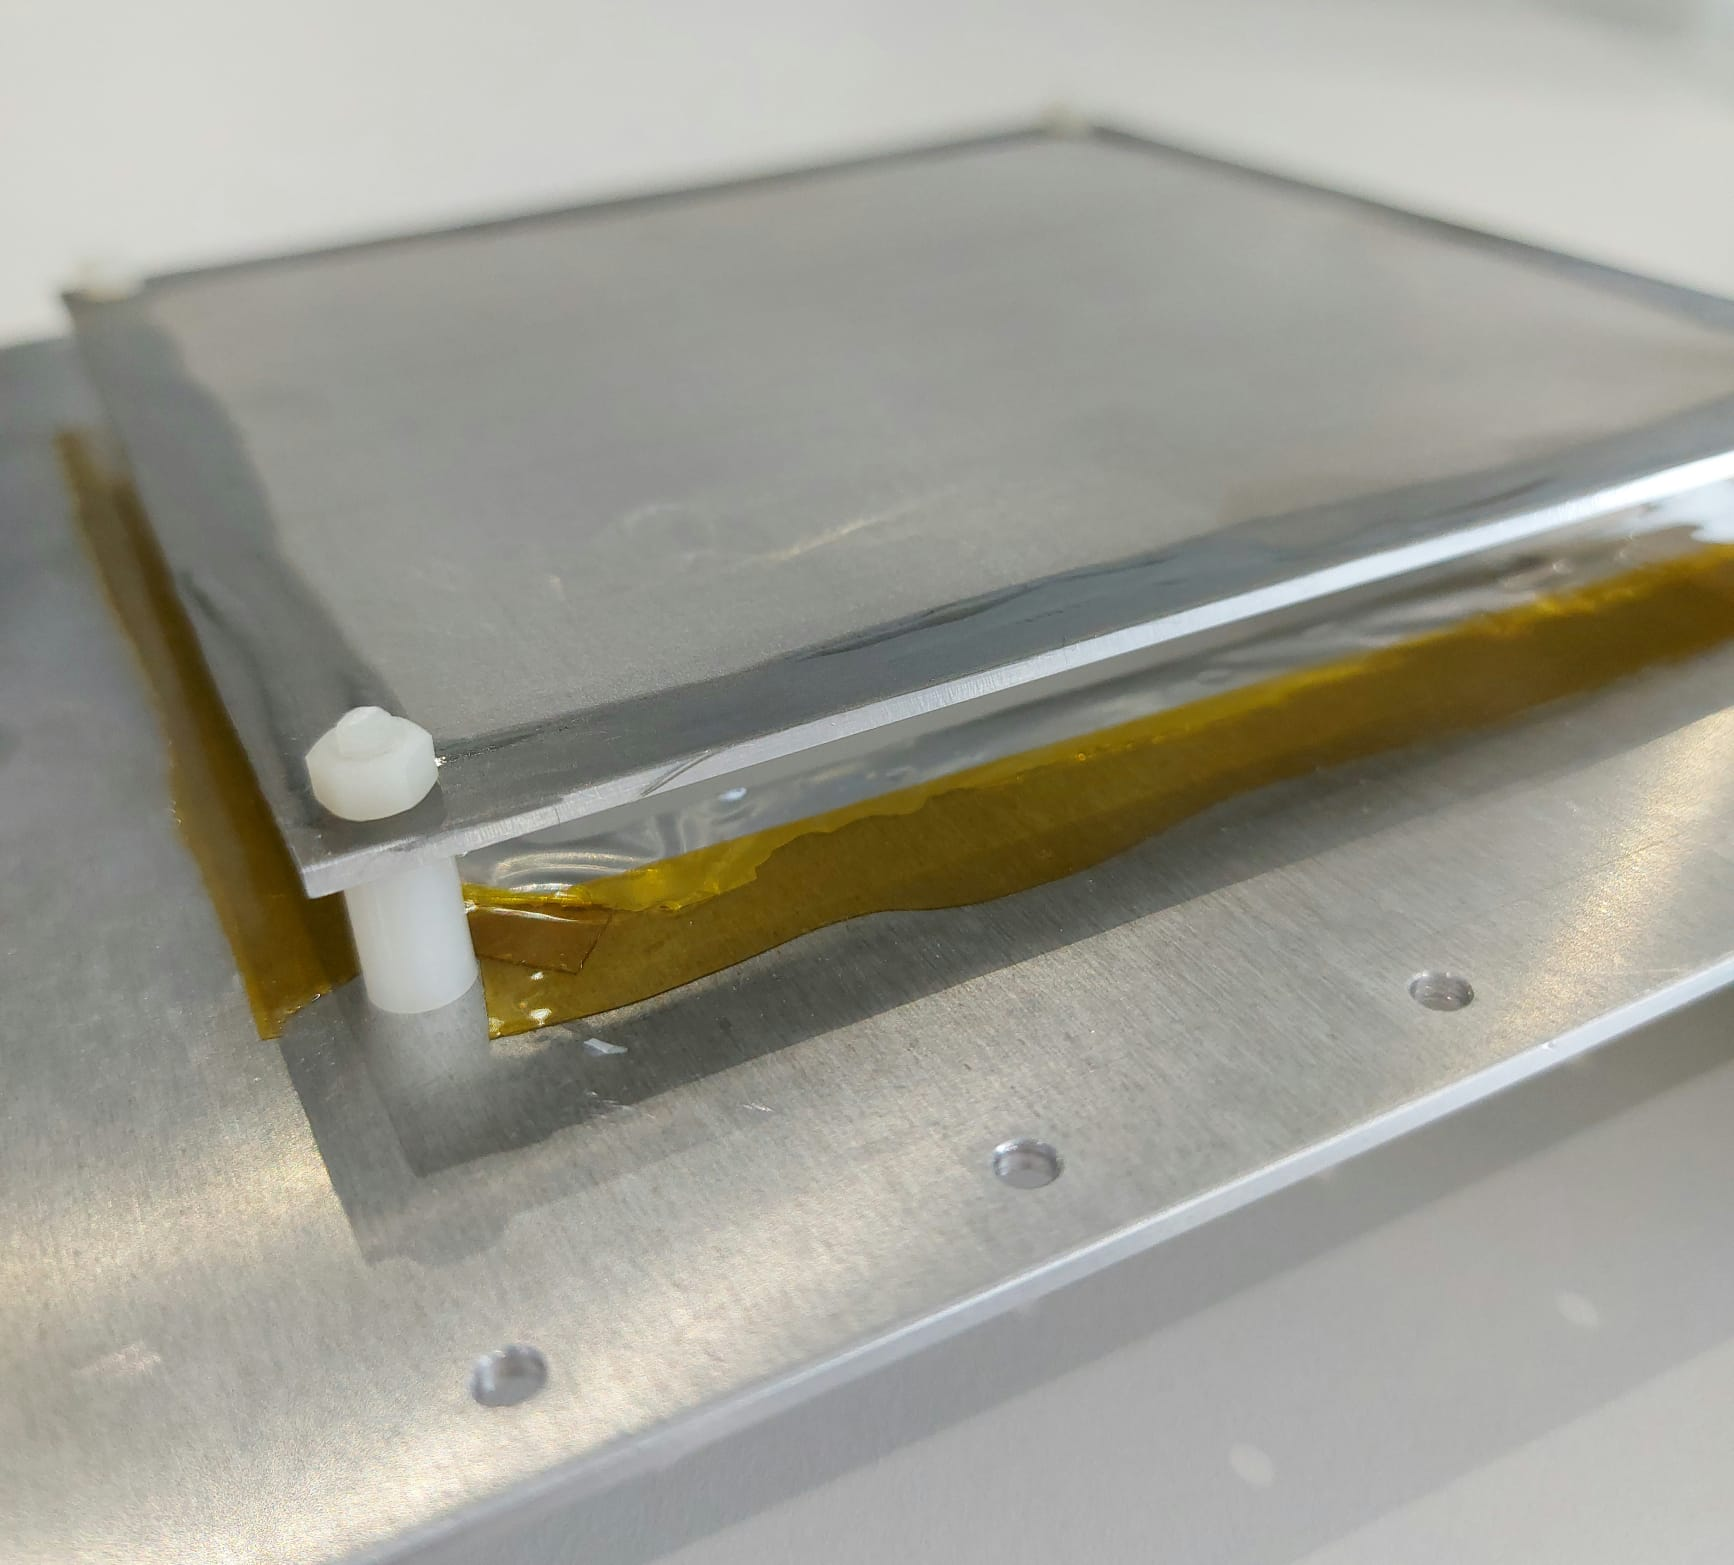
\includegraphics[width=\linewidth]{figures/micromegas_cover.jpeg}
        \caption{Cathode mesh on the upper part of the micromegas.}
        \label{fig:micromegas_cover}
    \end{subfigure}
    \begin{subfigure}{0.62\textwidth}
      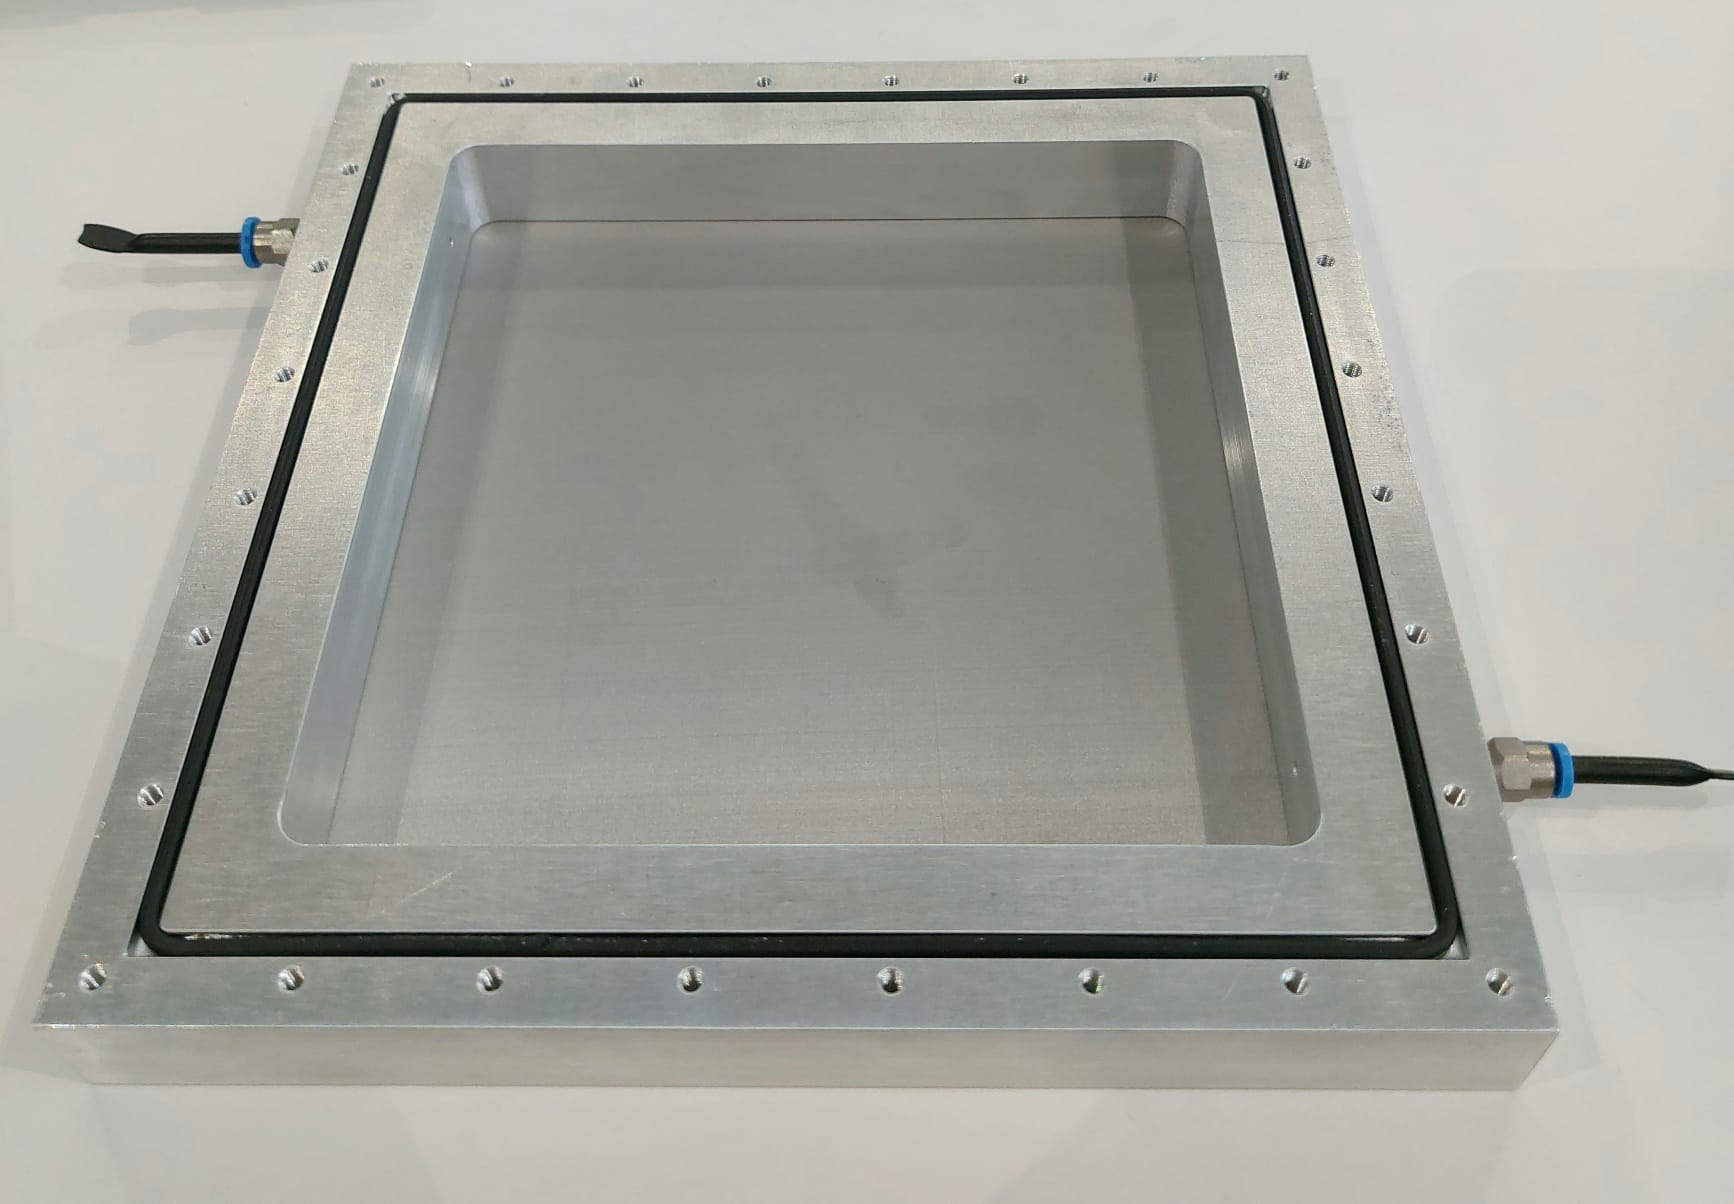
\includegraphics[width=\linewidth]{figures/micromegas_base_top.jpeg}
      \caption{Bottom part of the micromegas with the mesh.}
      \label{fig:micromegas_base}
    \end{subfigure}
    \begin{subfigure}{0.36\textwidth}
        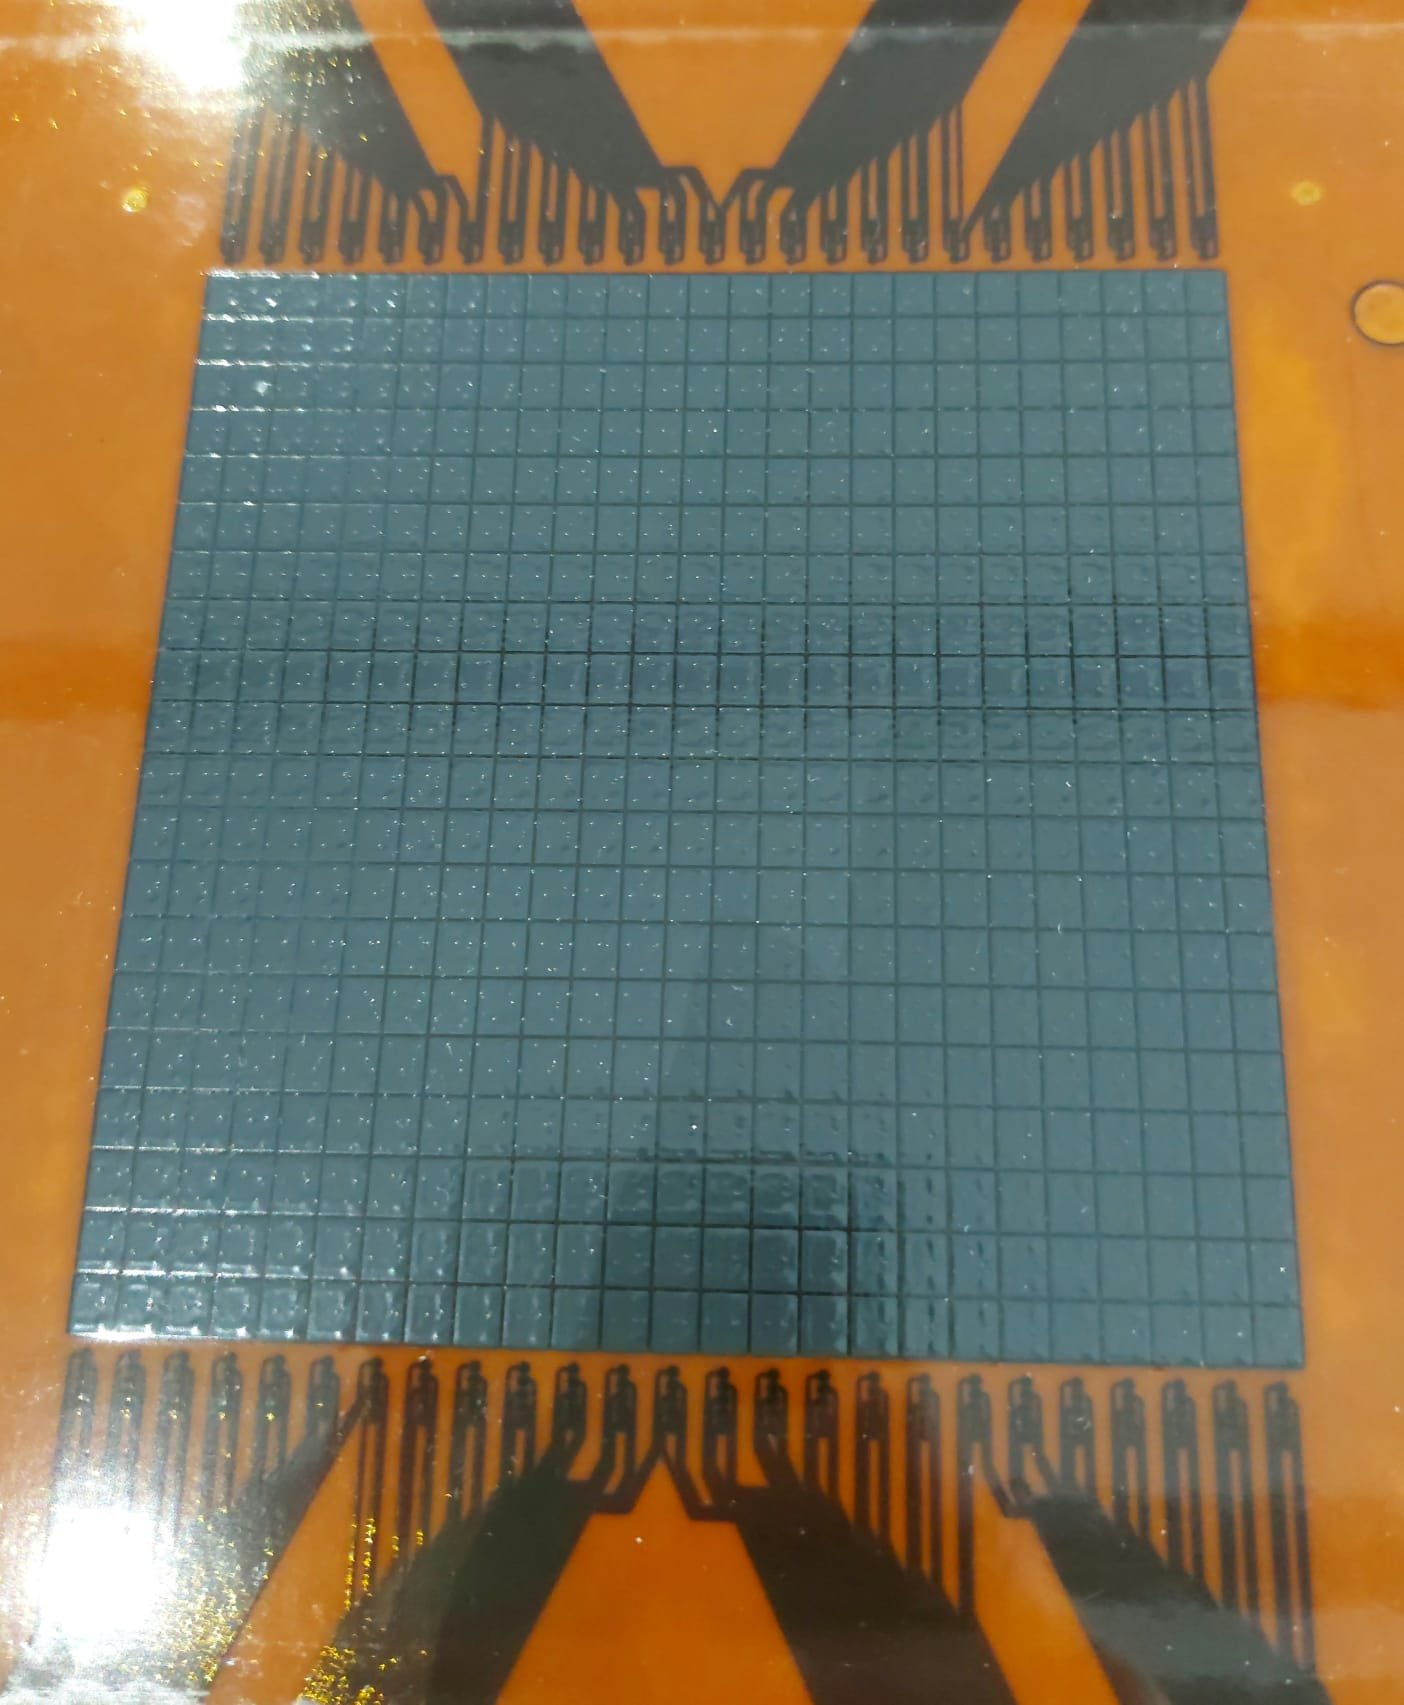
\includegraphics[width=\linewidth]{figures/micromegas_strips.jpeg}
        \caption{Grid structure of the anode strips.}
        \label{fig:micromegas_strips}
    \end{subfigure}
    \caption{Pictures of the disassembled micromegas detector.}
    \label{fig:mircro_wow}
\end{figure}



\clearpage
\section{Gaussian Distributions of Multiple Scattering for Observed Materials}
\renewcommand{\thefigure}{\Alph{section}\arabic{figure}}
\setcounter{figure}{0}
\renewcommand{\thetable}{\Alph{section}\arabic{table}}
\setcounter{table}{0}


\begin{figure}[h]
    \centering
    \begin{subfigure}{0.49\textwidth}
        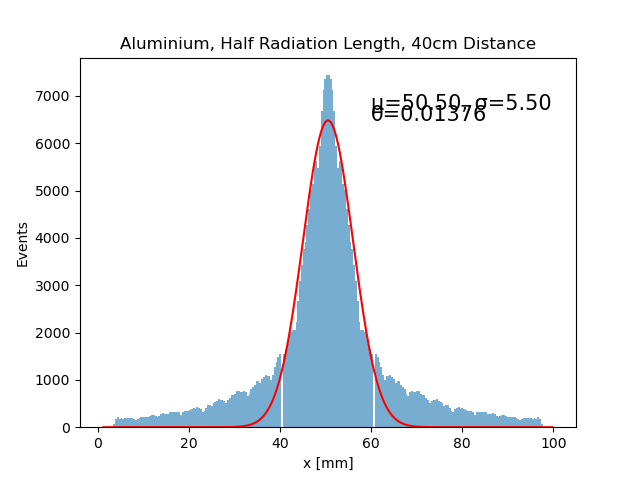
\includegraphics[width=\textwidth]{../src/elsa/finished_plots/Aluminium, Half Radiation Length, 40cm Distance.png}
        \caption{$x\approx\frac{X_0}{2}$}
    \end{subfigure}
    \begin{subfigure}{0.49\textwidth}
        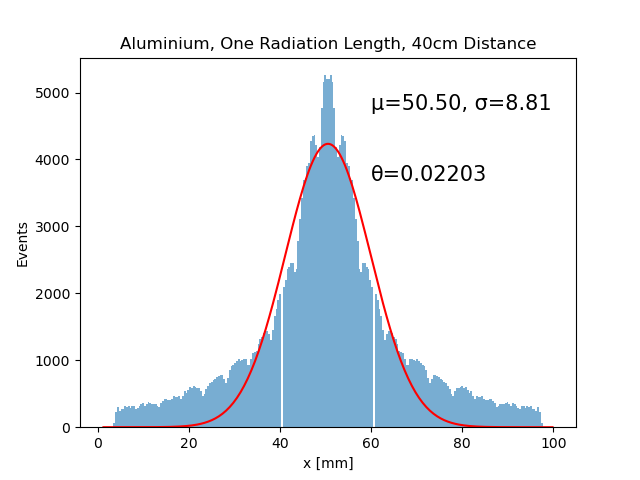
\includegraphics[width=\textwidth]{../src/elsa/finished_plots/Aluminium, One Radiation Length, 40cm Distance.png}
        \caption{$x\approx X_0$}
    \end{subfigure}
    \begin{subfigure}{0.49\textwidth}
        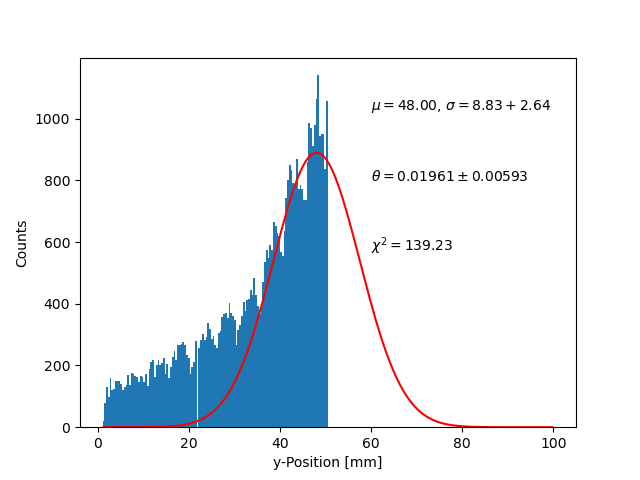
\includegraphics[width=\textwidth]{../src/elsa/finished_plots/Aluminium, Two Radiation Lengths, 40cm Distance.png}
        \caption{$x\approx2\cdot X_0$}
    \end{subfigure}
    \begin{subfigure}{0.49\textwidth}
        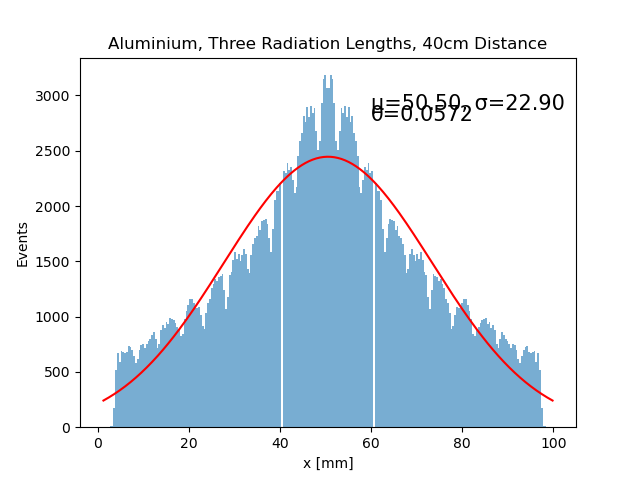
\includegraphics[width=\textwidth]{../src/elsa/finished_plots/Aluminium, Three Radiation Lengths, 40cm Distance.png}
        \caption{$x\approx3\cdot X_0$}
    \end{subfigure}
    \caption{Counted hits for aluminium of different thicknesses $x$.}
    \label{fig:alu_gaus}
\end{figure}

\begin{figure}[h]
    \centering
    \begin{subfigure}{0.49\textwidth}
        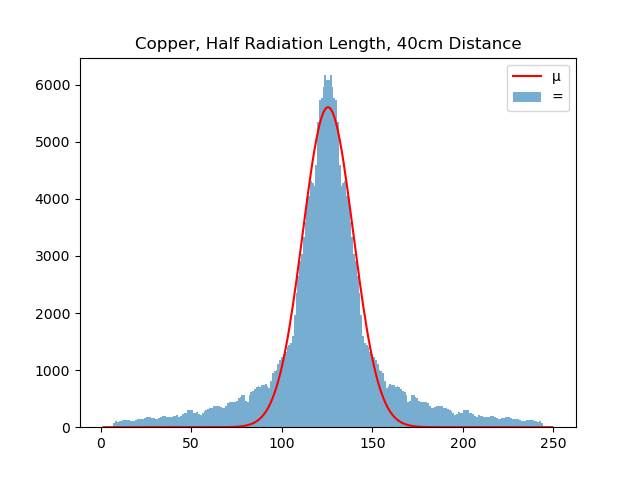
\includegraphics[width=\textwidth]{../src/elsa/finished_plots/Copper, Half Radiation Length, 40cm Distance.png}
        \caption{$x\approx\frac{X_0}{2}$}
    \end{subfigure}
    \begin{subfigure}{0.49\textwidth}
        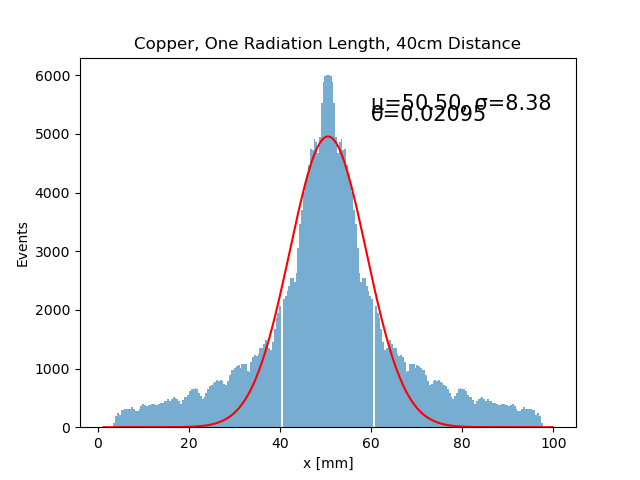
\includegraphics[width=\textwidth]{../src/elsa/finished_plots/Copper, One Radiation Length, 40cm Distance.png}
        \caption{$x\approx X_0$}
    \end{subfigure}
    \begin{subfigure}{0.49\textwidth}
        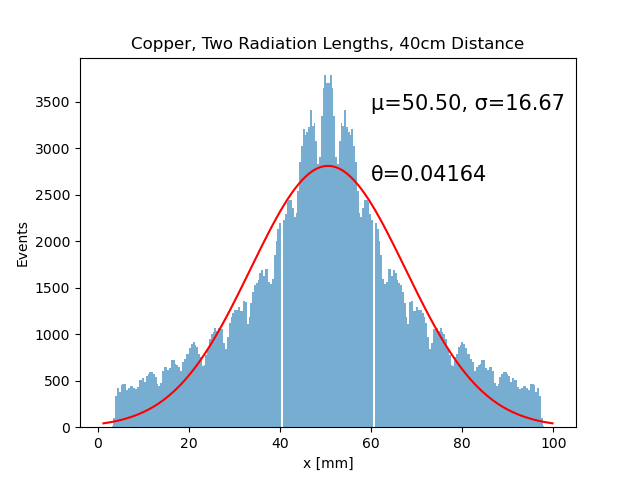
\includegraphics[width=\textwidth]{../src/elsa/finished_plots/Copper, Two Radiation Lengths, 40cm Distance.png}
        \caption{$x\approx2\cdot X_0$}
    \end{subfigure}
    \begin{subfigure}{0.49\textwidth}
        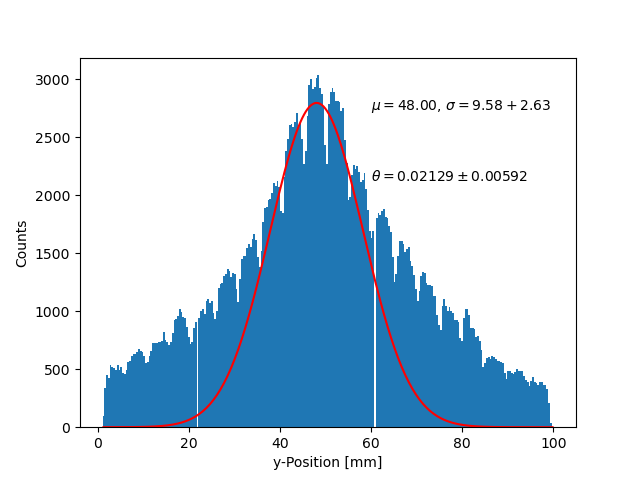
\includegraphics[width=\textwidth]{../src/elsa/finished_plots/Copper, Three Radiation Lengths, 40cm Distance.png}
        \caption{$x\approx3\cdot X_0$}
    \end{subfigure}
    \caption{Counted hits for copper of different thicknesses $x$.}
    \label{fig:cop_gaus}
\end{figure}



%-----------------------------------------------------------------------------------------------------------------------------

\clearpage
% \section{Analysis ELSA (\textbf{temporary information})}
% Here is a quick rundown of how the analysis for ELSA works.
 
% The way that the data taking works is that the detector triggers about every $\SI{25}{ns}$ and reads all strips.
% It needs some time to reset and then does it again.
% For ELSA data will be lost at downtime and the detector will basically trigger continuously because of the steady electron beam.

% The data will be such that one event (i.e.\ one trigger) contains (most probably) multiple hits (i.e.\ multiple strips fire / register a hit).
% Ideally, one would like only a single electron registered as a single hit.
% This poses a problem because there are many different reasons for the undesired multiple hits.
% \begin{enumerate}[label=\arabic*)]
%   \item There is a certain noise on the detector, which will be registered as a hit, but this only deposits very little charge.
%     To filter these events there is a certain charge threshold.
%   \item It is possible, that a beam-electron creates a $\delta $-electron in the material and both hit the detector.
%     This will be seen as two separate hits.
%   \item The electron has a very high energy and as it travels through the air, it is possible that it interacts with the air molecules.
%     This interaction could be inelastic scattering, which would result in a Hadron shower (most likely pions) on the detector.
%     This is seen (often) as a single hit (which is the electron; this hit can be very far from the expected distribution because it scattered under a higher angle) and a bunch of hits close together (Hadrons).
%     To filter these events one can count the number of independent strip(s) that fired.
%     Independence here means a strip or multiple strips next to each other give a signal and the adjacent strips to the left and right give none.
%     These strips are called clusters.
%     For example: \\\texttt{...|...||......||||..|.||.|..}\\
%     would be 6 clusters.
%     If the number of clusters in a single event is greater than a certain number $x$ (currently $x=2$), then this event will be left out.
% \end{enumerate}
% There will be a number of histograms, this includes: x and y strip events, clusters, cluster size, xy hitman etc.\
 
% For the analysis a Gaussian curve is fitted to the histogram: y strip events.
% The x strips don't work well (probably detector issue and the beam has an elliptic profile).
% The standard deviation of the curve is related to $\theta $ via $\tan \theta =\tfrac{\sigma }{d}$ with $d$ the distance between the target and the detector.
% First calculations with this formula are in the right order of magnitude.
% This will probably work better with a more precise filtering of the available data.
 
% To evaluate the theory, $$\theta _\text{exp}=\arctan\left(\dfrac{\sigma }{d}\right)$$ is plotted against $$\theta _\text{theo}=\text{const}\,\sqrt[]{\dfrac{x}{x_0}}\left(1+0.038\ln\left(\dfrac{x}{x_0}\right)\right).$$
% This should give a linear correlation between these two values thus verifying the proportionality i.e.\ the theory.
% \textbf{Currently there is no correlation at all between these two so WIP.}
 
% \bibliography{refs}
\newpage
\begin{thebibliography}{9}

\bibitem{Micromegas}
LMU München: Micromegas and GEMs: 
\href{https://www.etp.physik.uni-muenchen.de/research/detector-development/mm-and-gems/index.html}{https://www.etp.physik.uni-muenchen.de/...}
\bibitem{Highland}
Timothy Carlisle Oxford: Multiplie Scattering: 
\href{https://indico.cern.ch/event/190654/contributions/345614/attachments/270741/378860/CM33_ScatteringOverview.pdf}{https://indico.cern.ch/...}
\bibitem{Highland2}
Havard University: Multiplie Scattering: 
\href{https://gray.mgh.harvard.edu/media/com_dpattachments/attachments/com_content.article/Techniques-of-Proton-Radiotherapy-06-Multiple-Scattering.pdf}{https://gray.mgh.harvard.edu/...}
\bibitem{Scint}
EBSCO: Scintillators – Research Starter on Physics: 
\href{https://www.ebsco.com/research-starters/physics/scintillators}{https://www.ebsco.com/research-starters/...}
\bibitem{Micromega}
Dr. Saime Gürbüz \& Dr. Kristof Schmieden: Micromegas-Setup: 
\href{https://ecampus.uni-bonn.de/ilias.php?baseClass=ilrepositorygui&cmd=sendfile&ref_id=3786906}{https://ecampus.uni-bonn.de/...}
\bibitem{APV}
Lichtenberg Research Group: Micromegas Introduction: 
\href{https://ecampus.uni-bonn.de/ilias.php?baseClass=ilrepositorygui&cmd=sendfile&ref_id=3787243}{https://ecampus.uni-bonn.de/...}
\bibitem{mmDAQ}
CERN Indico: mmDAQ: 
\href{https://indico.cern.ch/event/240381/contributions/1554638/attachments/406597/564873/20130307-mmdaq1-flow-review-1.pdf}{https://indico.cern.ch/...}
\bibitem{muon}
Particle Data Group: Muon Properties: 
\href{https://pdg.lbl.gov/2023/listings/rpp2023-list-muon.pdf}{https://pdg.lbl.gov/...}
\bibitem{muonsea}
Steve Kliewer: Cosmic Ray Experiment:
\href{https://cosmic.lbl.gov/SKliewer/Cosmic_Rays/Muons.htm}{https://cosmic.lbl.gov/SKliewer/Cosmic\_Rays/Muons.htm}
\bibitem{ELSA}
Universität Bonn, PI: ELSA:
\href{https://www-elsa.physik.uni-bonn.de/}{https://www-elsa.physik.uni-bonn.de/}
\bibitem{radlength}
CERN: Radiationlength:
\href{https://cds.cern.ch/record/1279627/files/PH-EP-Tech-Note-2010-013.pdf}{https://cds.cern.ch/record/1279627/files/PH-EP-Tech-Note-2010-013.pdf}


\end{thebibliography}

\end{document}
